% ============================================================
% INFORME FINAL DE TESINA — formato APA 7.ª edición (trabajo de estudiante)
% Compilar con pdfLaTeX + Biber (en Overleaf: Menu → Compiler: pdfLaTeX; se usa Biber
% automáticamente al detectar biblatex). Requiere referencias.bib en la misma carpeta.
% Entrega: 29 de octubre de 2026.
% ============================================================
\documentclass[12pt,a4paper,oneside]{report}

% ------------------------------------------------------------
% IDIOMA, TIPOGRAFÍA Y PÁGINA (APA 7, sección 2.19–2.24)
% ------------------------------------------------------------
\usepackage[T1]{fontenc}
\usepackage[utf8]{inputenc}
\usepackage[english,spanish,es-tabla,es-nodecimaldot,es-noindentfirst]{babel}  % español idioma principal (último de la lista); inglés para el Abstract
\usepackage{newtxtext,newtxmath}          % Times, 12 pt
\usepackage[margin=2.54cm]{geometry}      % márgenes de 2,54 cm en los cuatro lados
\usepackage{setspace}
\doublespacing                            % doble espacio en todo el cuerpo
\usepackage{ragged2e}                     % alineado a la izquierda, sin justificar
\setlength{\RaggedRightParindent}{1.27cm} % sangría de primera línea de 1,27 cm
\setlength{\parindent}{1.27cm}
\setlength{\parskip}{0pt}
\usepackage{microtype}
\usepackage{csquotes}

% ------------------------------------------------------------
% TABLAS, FIGURAS Y LISTAS
% ------------------------------------------------------------
\usepackage{graphicx}
\usepackage{booktabs}
\usepackage{longtable}
\usepackage{tabularx}
\usepackage{array}
\usepackage{float}
\usepackage{threeparttable}
\usepackage{enumitem}
\setlist{nosep,leftmargin=1.27cm}
\usepackage{amsmath}
\usepackage{url}

% Rótulos APA: «Tabla 1» en negrita, título en cursiva en la línea siguiente, ambos arriba y
% alineados a la izquierda; numeración correlativa en todo el documento.
\usepackage{caption}
\captionsetup{labelfont=bf,textfont=it,labelsep=newline,justification=RaggedRight,
  singlelinecheck=false,skip=6pt,font={stretch=1.0}}
\captionsetup[table]{position=top}
\captionsetup[figure]{position=top}
\usepackage{chngcntr}
\counterwithout{table}{chapter}
\counterwithout{figure}{chapter}
% Nota de tabla al pie, en el formato APA («Nota.» en cursiva).
\newcommand{\notatabla}[1]{\par\vspace{2pt}{\singlespacing\small\RaggedRight\noindent\textit{Nota.} #1\par}}

% ------------------------------------------------------------
% ENCABEZADOS APA
%   Nivel 1 (capítulo): centrado, negrita.  Nivel 2 (section): izquierda, negrita.
%   Nivel 3 (subsection): izquierda, negrita cursiva.
% Los capítulos conservan la numeración del índice propuesto en el plan de trabajo; las
% secciones no se numeran (APA 7, sección 2.27).
% ------------------------------------------------------------
\usepackage{titlesec}
\setcounter{secnumdepth}{-1}
\titleformat{\chapter}[block]{\normalfont\normalsize\bfseries\filcenter}{}{0pt}{}
\titlespacing*{\chapter}{0pt}{0pt}{12pt}
\titleformat{\section}{\normalfont\normalsize\bfseries}{}{0pt}{}
\titlespacing*{\section}{0pt}{12pt}{0pt}
\titleformat{\subsection}{\normalfont\normalsize\bfseries\itshape}{}{0pt}{}
\titlespacing*{\subsection}{0pt}{12pt}{0pt}
% Los capítulos se numeran a mano para que el título y el índice digan «Capítulo N.» una sola vez.
\newcommand{\capitulo}[1]{\stepcounter{chapter}%
  \chapter*{Capítulo \arabic{chapter}. #1}%
  \addcontentsline{toc}{chapter}{Capítulo \arabic{chapter}. #1}}

% Número de página arriba a la derecha (APA 7, sección 2.18); sin encabezado corrido.
\usepackage{fancyhdr}
\setlength{\headheight}{14.5pt}      % evita la advertencia de fancyhdr
\pagestyle{fancy}
\fancyhf{}
\fancyhead[R]{\thepage}
\renewcommand{\headrulewidth}{0pt}
\fancypagestyle{plain}{\fancyhf{}\fancyhead[R]{\thepage}\renewcommand{\headrulewidth}{0pt}}

% ------------------------------------------------------------
% REFERENCIAS APA 7
% ------------------------------------------------------------
\usepackage[style=apa,backend=biber]{biblatex}
\addbibresource{referencias.bib}

\usepackage[hidelinks]{hyperref}
% Cifras del informe generadas desde los JSON (informe/generar_cifras.py); ver informe/LEEME.md
% generado por informe/generar_cifras.py, no editar.
% Cada macro es una cifra del informe, formateada en español (coma decimal). Usar como \Macro{} o \Macro\ 
% (con llaves vacías para que no se coma el espacio siguiente).
% Correspondencia macro = fuente (también en informe/cifras_lista.md):
%   \ClipsTotal = comparacion/resultados/validacion_por_sesion.json; comparacion/reserva_caballos.json
%   \ClipsDesarrollo = comparacion/resultados/validacion_por_sesion.json (intervalos.todo.clips)
%   \ClipsReserva = comparacion/resultados/fusion_tardia_pose_visual__reserva.json (clips)
%   \CaballosTotal = comparacion/reserva_caballos.json
%   \CaballosDesarrollo = comparacion/reserva_caballos.json (desarrollo)
%   \CaballosReserva = comparacion/reserva_caballos.json (reserva)
%   \VideosTotal = comparacion/sesiones_resumen.json
%   \SesionesTotal = comparacion/sesiones_de_filmacion.csv (sesion_confirmada)
%   \SesionesEvaluadas = comparacion/resultados/validacion_por_sesion.json (plan.evaluadas)
%   \ClipsLimpioDesarrollo = comparacion/resultados/validacion_por_sesion.json (intervalos.limpio)
%   \CaballosLimpioDesarrollo = comparacion/resultados/validacion_por_sesion.json (intervalos.limpio)
%   \ClipsLimpioReserva = comparacion/DECISION.md (reserva, subconjunto limpio)
%   \CriterioLimpio = comparacion/resultados/*.json (limpio.criterio)
%   \ClipsDevDisg = comparacion/resultados/fusion...json (matriz_confusion_suma / 5)
%   \ClipsReservaDisg = comparacion/resultados/fusion...__reserva.json (matriz)
%   \ClipsLimpioDisg = comparacion/resultados/fusion...json (limpio.clips_por_clase)
%   \ClipsDevInt = comparacion/resultados/fusion...json (matriz_confusion_suma / 5)
%   \ClipsReservaInt = comparacion/resultados/fusion...__reserva.json (matriz)
%   \ClipsLimpioInt = comparacion/resultados/fusion...json (limpio.clips_por_clase)
%   \ClipsDevSer = comparacion/resultados/fusion...json (matriz_confusion_suma / 5)
%   \ClipsReservaSer = comparacion/resultados/fusion...__reserva.json (matriz)
%   \ClipsLimpioSer = comparacion/resultados/fusion...json (limpio.clips_por_clase)
%   \Repeticiones = comparacion/resultados/*.json (R)
%   \Folds = comparacion/resultados/*.json (K)
%   \Evaluaciones = comparacion/resultados/*.json
%   \ReplicasBootstrap = comparacion/resultados/comparaciones_pareadas.json
%   \SemillaBootstrap = comparacion/resultados/comparaciones_pareadas.json
%   \ClipsTrainSesionMin = comparacion/resultados/validacion_por_sesion.json (plan.evaluadas)
%   \ClipsTrainSesionMax = comparacion/resultados/validacion_por_sesion.json (plan.evaluadas)
%   \ClipsTrainPerdidos = comparacion/resultados/validacion_por_sesion.json (plan)
%   \ClipsTrainPerdidosMedia = comparacion/resultados/validacion_por_sesion.json (plan)
%   \PoseRasgos = comparacion/resultados/fusion...json (descripcion)
%   \Fotogramas = equinos/comparacion.py (Datos: 16 frames por clip)
%   \PesoPose = comparacion/DECISION.md (peso elegido en validación interna)
%   \PesoFoldsA = comparacion/DECISION.md
%   \PesoFoldsTotal = comparacion/DECISION.md
%   \PesoPoseUno = comparacion/DECISION.md
%   \FusionDevF = comparacion/resultados/fusion_tardia_pose_visual.json (global.f1_macro.media)
%   \FusionDevDE = comparacion/resultados/fusion_tardia_pose_visual.json (global.f1_macro.desvio)
%   \FusionDevAcc = comparacion/resultados/fusion_tardia_pose_visual.json (global.accuracy.media)
%   \FusionDevAccDE = comparacion/resultados/fusion_tardia_pose_visual.json (global.accuracy.desvio)
%   \FusionLimpioF = comparacion/resultados/fusion_tardia_pose_visual.json (limpio.f1_macro_oof_por_repeticion.media)
%   \FusionLimpioDE = comparacion/resultados/fusion_tardia_pose_visual.json (limpio.f1_macro_oof_por_repeticion.desvio)
%   \FusionGap = comparacion/resultados/fusion_tardia_pose_visual.json (global.gap_train_test_f1.media)
%   \FusionGapDE = comparacion/resultados/fusion_tardia_pose_visual.json (global.gap_train_test_f1.desvio)
%   \FusionTrainF = comparacion/resultados/fusion_tardia_pose_visual.json (global.f1_macro_train.media)
%   \FusionAgrupF = comparacion/resultados/comparaciones_pareadas.json (f1_a/f1_b)
%   \FusionAgrupIC = comparacion/resultados/comparaciones_pareadas.json
%   \FusionAgrupLimpioF = comparacion/resultados/comparaciones_pareadas.json
%   \FusionAgrupLimpioIC = comparacion/resultados/comparaciones_pareadas.json
%   \FusionSesionF = comparacion/resultados/validacion_por_sesion.json (intervalos.todo.f1_agrupado)
%   \FusionSesionIC = comparacion/resultados/validacion_por_sesion.json
%   \FusionSesionAcc = comparacion/resultados/validacion_por_sesion.json (candidatos.*.metricas.accuracy)
%   \FusionSesionLimpioF = comparacion/resultados/validacion_por_sesion.json (intervalos.limpio.f1_agrupado)
%   \FusionSesionLimpioIC = comparacion/resultados/validacion_por_sesion.json
%   \FusionSesionCaida = 5×4 agrupado − sesión (calculado)
%   \FusionSesionCaidaLimpio = ídem, limpio
%   \FusionDevFDisg = comparacion/resultados/fusion_tardia_pose_visual.json (global.por_clase.Disgustado.f1.media)
%   \FusionDevFDisgDE = comparacion/resultados/fusion_tardia_pose_visual.json (global.por_clase.Disgustado.f1.desvio)
%   \FusionSesionFDisg = comparacion/resultados/validacion_por_sesion.json (candidatos.*.metricas.f1.Disgustado)
%   \FusionDevFInt = comparacion/resultados/fusion_tardia_pose_visual.json (global.por_clase.Interesado.f1.media)
%   \FusionDevFIntDE = comparacion/resultados/fusion_tardia_pose_visual.json (global.por_clase.Interesado.f1.desvio)
%   \FusionSesionFInt = comparacion/resultados/validacion_por_sesion.json (candidatos.*.metricas.f1.Interesado)
%   \FusionDevFSer = comparacion/resultados/fusion_tardia_pose_visual.json (global.por_clase.Sereno.f1.media)
%   \FusionDevFSerDE = comparacion/resultados/fusion_tardia_pose_visual.json (global.por_clase.Sereno.f1.desvio)
%   \FusionSesionFSer = comparacion/resultados/validacion_por_sesion.json (candidatos.*.metricas.f1.Sereno)
%   \RFPoseDevF = comparacion/resultados/rf_pose_tipo_simba.json (global.f1_macro.media)
%   \RFPoseDevDE = comparacion/resultados/rf_pose_tipo_simba.json (global.f1_macro.desvio)
%   \RFPoseDevAcc = comparacion/resultados/rf_pose_tipo_simba.json (global.accuracy.media)
%   \RFPoseDevAccDE = comparacion/resultados/rf_pose_tipo_simba.json (global.accuracy.desvio)
%   \RFPoseLimpioF = comparacion/resultados/rf_pose_tipo_simba.json (limpio.f1_macro_oof_por_repeticion.media)
%   \RFPoseLimpioDE = comparacion/resultados/rf_pose_tipo_simba.json (limpio.f1_macro_oof_por_repeticion.desvio)
%   \RFPoseGap = comparacion/resultados/rf_pose_tipo_simba.json (global.gap_train_test_f1.media)
%   \RFPoseGapDE = comparacion/resultados/rf_pose_tipo_simba.json (global.gap_train_test_f1.desvio)
%   \RFPoseTrainF = comparacion/resultados/rf_pose_tipo_simba.json (global.f1_macro_train.media)
%   \RFPoseAgrupF = comparacion/resultados/comparaciones_pareadas.json (f1_a/f1_b)
%   \RFPoseAgrupIC = comparacion/resultados/comparaciones_pareadas.json
%   \RFPoseAgrupLimpioF = comparacion/resultados/comparaciones_pareadas.json
%   \RFPoseAgrupLimpioIC = comparacion/resultados/comparaciones_pareadas.json
%   \RFPoseSesionF = comparacion/resultados/validacion_por_sesion.json (intervalos.todo.f1_agrupado)
%   \RFPoseSesionIC = comparacion/resultados/validacion_por_sesion.json
%   \RFPoseSesionAcc = comparacion/resultados/validacion_por_sesion.json (candidatos.*.metricas.accuracy)
%   \RFPoseSesionLimpioF = comparacion/resultados/validacion_por_sesion.json (intervalos.limpio.f1_agrupado)
%   \RFPoseSesionLimpioIC = comparacion/resultados/validacion_por_sesion.json
%   \RFPoseSesionCaida = 5×4 agrupado − sesión (calculado)
%   \RFPoseSesionCaidaLimpio = ídem, limpio
%   \RFPoseDevFDisg = comparacion/resultados/rf_pose_tipo_simba.json (global.por_clase.Disgustado.f1.media)
%   \RFPoseDevFDisgDE = comparacion/resultados/rf_pose_tipo_simba.json (global.por_clase.Disgustado.f1.desvio)
%   \RFPoseSesionFDisg = comparacion/resultados/validacion_por_sesion.json (candidatos.*.metricas.f1.Disgustado)
%   \RFPoseDevFInt = comparacion/resultados/rf_pose_tipo_simba.json (global.por_clase.Interesado.f1.media)
%   \RFPoseDevFIntDE = comparacion/resultados/rf_pose_tipo_simba.json (global.por_clase.Interesado.f1.desvio)
%   \RFPoseSesionFInt = comparacion/resultados/validacion_por_sesion.json (candidatos.*.metricas.f1.Interesado)
%   \RFPoseDevFSer = comparacion/resultados/rf_pose_tipo_simba.json (global.por_clase.Sereno.f1.media)
%   \RFPoseDevFSerDE = comparacion/resultados/rf_pose_tipo_simba.json (global.por_clase.Sereno.f1.desvio)
%   \RFPoseSesionFSer = comparacion/resultados/validacion_por_sesion.json (candidatos.*.metricas.f1.Sereno)
%   \MILDevF = comparacion/resultados/mil_multimodal_corregido.json (global.f1_macro.media)
%   \MILDevDE = comparacion/resultados/mil_multimodal_corregido.json (global.f1_macro.desvio)
%   \MILDevAcc = comparacion/resultados/mil_multimodal_corregido.json (global.accuracy.media)
%   \MILDevAccDE = comparacion/resultados/mil_multimodal_corregido.json (global.accuracy.desvio)
%   \MILLimpioF = comparacion/resultados/mil_multimodal_corregido.json (limpio.f1_macro_oof_por_repeticion.media)
%   \MILLimpioDE = comparacion/resultados/mil_multimodal_corregido.json (limpio.f1_macro_oof_por_repeticion.desvio)
%   \MILGap = comparacion/resultados/mil_multimodal_corregido.json (global.gap_train_test_f1.media)
%   \MILGapDE = comparacion/resultados/mil_multimodal_corregido.json (global.gap_train_test_f1.desvio)
%   \MILTrainF = comparacion/resultados/mil_multimodal_corregido.json (global.f1_macro_train.media)
%   \MILAgrupF = comparacion/resultados/comparaciones_pareadas.json (f1_a/f1_b)
%   \MILAgrupIC = comparacion/resultados/comparaciones_pareadas.json
%   \MILAgrupLimpioF = comparacion/resultados/comparaciones_pareadas.json
%   \MILAgrupLimpioIC = comparacion/resultados/comparaciones_pareadas.json
%   \MILSesionF = comparacion/resultados/validacion_por_sesion.json (intervalos.todo.f1_agrupado)
%   \MILSesionIC = comparacion/resultados/validacion_por_sesion.json
%   \MILSesionAcc = comparacion/resultados/validacion_por_sesion.json (candidatos.*.metricas.accuracy)
%   \MILSesionLimpioF = comparacion/resultados/validacion_por_sesion.json (intervalos.limpio.f1_agrupado)
%   \MILSesionLimpioIC = comparacion/resultados/validacion_por_sesion.json
%   \MILSesionCaida = 5×4 agrupado − sesión (calculado)
%   \MILSesionCaidaLimpio = ídem, limpio
%   \MILDevFDisg = comparacion/resultados/mil_multimodal_corregido.json (global.por_clase.Disgustado.f1.media)
%   \MILDevFDisgDE = comparacion/resultados/mil_multimodal_corregido.json (global.por_clase.Disgustado.f1.desvio)
%   \MILSesionFDisg = comparacion/resultados/validacion_por_sesion.json (candidatos.*.metricas.f1.Disgustado)
%   \MILDevFInt = comparacion/resultados/mil_multimodal_corregido.json (global.por_clase.Interesado.f1.media)
%   \MILDevFIntDE = comparacion/resultados/mil_multimodal_corregido.json (global.por_clase.Interesado.f1.desvio)
%   \MILSesionFInt = comparacion/resultados/validacion_por_sesion.json (candidatos.*.metricas.f1.Interesado)
%   \MILDevFSer = comparacion/resultados/mil_multimodal_corregido.json (global.por_clase.Sereno.f1.media)
%   \MILDevFSerDE = comparacion/resultados/mil_multimodal_corregido.json (global.por_clase.Sereno.f1.desvio)
%   \MILSesionFSer = comparacion/resultados/validacion_por_sesion.json (candidatos.*.metricas.f1.Sereno)
%   \BaseDevF = comparacion/resultados/baseline_logreg_media_frames.json (global.f1_macro.media)
%   \BaseDevDE = comparacion/resultados/baseline_logreg_media_frames.json (global.f1_macro.desvio)
%   \BaseDevAcc = comparacion/resultados/baseline_logreg_media_frames.json (global.accuracy.media)
%   \BaseDevAccDE = comparacion/resultados/baseline_logreg_media_frames.json (global.accuracy.desvio)
%   \BaseLimpioF = comparacion/resultados/baseline_logreg_media_frames.json (limpio.f1_macro_oof_por_repeticion.media)
%   \BaseLimpioDE = comparacion/resultados/baseline_logreg_media_frames.json (limpio.f1_macro_oof_por_repeticion.desvio)
%   \BaseGap = comparacion/resultados/baseline_logreg_media_frames.json (global.gap_train_test_f1.media)
%   \BaseGapDE = comparacion/resultados/baseline_logreg_media_frames.json (global.gap_train_test_f1.desvio)
%   \BaseTrainF = comparacion/resultados/baseline_logreg_media_frames.json (global.f1_macro_train.media)
%   \BaseAgrupF = comparacion/resultados/comparaciones_pareadas.json (f1_a/f1_b)
%   \BaseAgrupIC = comparacion/resultados/comparaciones_pareadas.json
%   \BaseAgrupLimpioF = comparacion/resultados/comparaciones_pareadas.json
%   \BaseAgrupLimpioIC = comparacion/resultados/comparaciones_pareadas.json
%   \BaseSesionF = comparacion/resultados/validacion_por_sesion.json (intervalos.todo.f1_agrupado)
%   \BaseSesionIC = comparacion/resultados/validacion_por_sesion.json
%   \BaseSesionAcc = comparacion/resultados/validacion_por_sesion.json (candidatos.*.metricas.accuracy)
%   \BaseSesionLimpioF = comparacion/resultados/validacion_por_sesion.json (intervalos.limpio.f1_agrupado)
%   \BaseSesionLimpioIC = comparacion/resultados/validacion_por_sesion.json
%   \BaseSesionCaida = 5×4 agrupado − sesión (calculado)
%   \BaseSesionCaidaLimpio = ídem, limpio
%   \BaseDevFDisg = comparacion/resultados/baseline_logreg_media_frames.json (global.por_clase.Disgustado.f1.media)
%   \BaseDevFDisgDE = comparacion/resultados/baseline_logreg_media_frames.json (global.por_clase.Disgustado.f1.desvio)
%   \BaseSesionFDisg = comparacion/resultados/validacion_por_sesion.json (candidatos.*.metricas.f1.Disgustado)
%   \BaseDevFInt = comparacion/resultados/baseline_logreg_media_frames.json (global.por_clase.Interesado.f1.media)
%   \BaseDevFIntDE = comparacion/resultados/baseline_logreg_media_frames.json (global.por_clase.Interesado.f1.desvio)
%   \BaseSesionFInt = comparacion/resultados/validacion_por_sesion.json (candidatos.*.metricas.f1.Interesado)
%   \BaseDevFSer = comparacion/resultados/baseline_logreg_media_frames.json (global.por_clase.Sereno.f1.media)
%   \BaseDevFSerDE = comparacion/resultados/baseline_logreg_media_frames.json (global.por_clase.Sereno.f1.desvio)
%   \BaseSesionFSer = comparacion/resultados/validacion_por_sesion.json (candidatos.*.metricas.f1.Sereno)
%   \FusionReservaF = comparacion/resultados/fusion_tardia_pose_visual__reserva.json (metricas.f1_macro)
%   \FusionReservaIC = comparacion/resultados/fusion_tardia_pose_visual__reserva.json (IC95 bootstrap por caballo)
%   \FusionReservaAcc = comparacion/resultados/fusion_tardia_pose_visual__reserva.json (metricas.accuracy)
%   \FusionReservaAccDec = comparacion/resultados/fusion_tardia_pose_visual__reserva.json (metricas.accuracy)
%   \FusionReservaLimpio = comparacion/resultados/fusion_tardia_pose_visual__reserva.json (limpio_f1_macro)
%   \FusionReservaFDisg = comparacion/resultados/fusion_tardia_pose_visual__reserva.json (metricas.f1.Disgustado)
%   \FusionReservaPrecDisg = comparacion/resultados/fusion_tardia_pose_visual__reserva.json (metricas.precision.Disgustado)
%   \FusionReservaRecDisg = comparacion/resultados/fusion_tardia_pose_visual__reserva.json (metricas.recall.Disgustado)
%   \FusionReservaFInt = comparacion/resultados/fusion_tardia_pose_visual__reserva.json (metricas.f1.Interesado)
%   \FusionReservaPrecInt = comparacion/resultados/fusion_tardia_pose_visual__reserva.json (metricas.precision.Interesado)
%   \FusionReservaRecInt = comparacion/resultados/fusion_tardia_pose_visual__reserva.json (metricas.recall.Interesado)
%   \FusionReservaFSer = comparacion/resultados/fusion_tardia_pose_visual__reserva.json (metricas.f1.Sereno)
%   \FusionReservaPrecSer = comparacion/resultados/fusion_tardia_pose_visual__reserva.json (metricas.precision.Sereno)
%   \FusionReservaRecSer = comparacion/resultados/fusion_tardia_pose_visual__reserva.json (metricas.recall.Sereno)
%   \ReservaAciertos = comparacion/resultados/fusion_tardia_pose_visual__reserva.json (traza de la matriz)
%   \DifFusionRFDev = comparacion/resultados/comparaciones_pareadas.json (fusion_tardia_pose_visual vs rf_pose_tipo_simba, todo)
%   \DifFusionRFDevIC = comparacion/resultados/comparaciones_pareadas.json
%   \DifFusionRFLimpio = comparacion/resultados/comparaciones_pareadas.json (fusion_tardia_pose_visual vs rf_pose_tipo_simba, limpio)
%   \DifFusionRFLimpioIC = comparacion/resultados/comparaciones_pareadas.json
%   \DifFusionRFSesion = comparacion/resultados/validacion_por_sesion.json (intervalos.todo.diferencia_vs_fusion...)
%   \DifFusionRFSesionIC = comparacion/resultados/validacion_por_sesion.json
%   \DifFusionRFSesionLimpio = comparacion/resultados/validacion_por_sesion.json (intervalos.limpio.diferencia_vs_fusion...)
%   \DifFusionRFSesionLimpioIC = comparacion/resultados/validacion_por_sesion.json
%   \DifFusionMILDev = comparacion/resultados/comparaciones_pareadas.json (fusion_tardia_pose_visual vs mil_multimodal_corregido, todo)
%   \DifFusionMILDevIC = comparacion/resultados/comparaciones_pareadas.json
%   \DifFusionMILLimpio = comparacion/resultados/comparaciones_pareadas.json (fusion_tardia_pose_visual vs mil_multimodal_corregido, limpio)
%   \DifFusionMILLimpioIC = comparacion/resultados/comparaciones_pareadas.json
%   \DifFusionMILSesion = comparacion/resultados/validacion_por_sesion.json (intervalos.todo.diferencia_vs_fusion...)
%   \DifFusionMILSesionIC = comparacion/resultados/validacion_por_sesion.json
%   \DifFusionMILSesionLimpio = comparacion/resultados/validacion_por_sesion.json (intervalos.limpio.diferencia_vs_fusion...)
%   \DifFusionMILSesionLimpioIC = comparacion/resultados/validacion_por_sesion.json
%   \DifFusionBaseDev = comparacion/resultados/comparaciones_pareadas.json (fusion_tardia_pose_visual vs baseline_logreg_media_frames, todo)
%   \DifFusionBaseDevIC = comparacion/resultados/comparaciones_pareadas.json
%   \DifFusionBaseLimpio = comparacion/resultados/comparaciones_pareadas.json (fusion_tardia_pose_visual vs baseline_logreg_media_frames, limpio)
%   \DifFusionBaseLimpioIC = comparacion/resultados/comparaciones_pareadas.json
%   \DifFusionBaseSesion = comparacion/resultados/validacion_por_sesion.json (intervalos.todo.diferencia_vs_fusion...)
%   \DifFusionBaseSesionIC = comparacion/resultados/validacion_por_sesion.json
%   \DifFusionBaseSesionLimpio = comparacion/resultados/validacion_por_sesion.json (intervalos.limpio.diferencia_vs_fusion...)
%   \DifFusionBaseSesionLimpioIC = comparacion/resultados/validacion_por_sesion.json
%   \DifRFMILDev = comparacion/resultados/comparaciones_pareadas.json (rf_pose_tipo_simba vs mil_multimodal_corregido, todo)
%   \DifRFMILDevIC = comparacion/resultados/comparaciones_pareadas.json
%   \DifRFMILLimpio = comparacion/resultados/comparaciones_pareadas.json (rf_pose_tipo_simba vs mil_multimodal_corregido, limpio)
%   \DifRFMILLimpioIC = comparacion/resultados/comparaciones_pareadas.json
%   \DifRFBaseDev = comparacion/resultados/comparaciones_pareadas.json (rf_pose_tipo_simba vs baseline_logreg_media_frames, todo)
%   \DifRFBaseDevIC = comparacion/resultados/comparaciones_pareadas.json
%   \DifRFBaseLimpio = comparacion/resultados/comparaciones_pareadas.json (rf_pose_tipo_simba vs baseline_logreg_media_frames, limpio)
%   \DifRFBaseLimpioIC = comparacion/resultados/comparaciones_pareadas.json
%   \ParClips = equinos.comparacion.Datos (clips de los caballos 123 y 169)
%   \ParRepsSeparado = comparacion/DECISION.md
%   \ParFusionAntes = calculado de predicciones_oof (291 clips)
%   \ParFusionDespues = calculado de predicciones_oof (sin los 5 clips)
%   \ParFusionDif = calculado
%   \ParRFAntes = calculado de predicciones_oof (291 clips)
%   \ParRFDespues = calculado de predicciones_oof (sin los 5 clips)
%   \ParRFDif = calculado
%   \ParMILAntes = calculado de predicciones_oof (291 clips)
%   \ParMILDespues = calculado de predicciones_oof (sin los 5 clips)
%   \ParMILDif = calculado
%   \ParBaseAntes = calculado de predicciones_oof (291 clips)
%   \ParBaseDespues = calculado de predicciones_oof (sin los 5 clips)
%   \ParBaseDif = calculado

\newcommand{\ClipsTotal}{359}
\newcommand{\ClipsDesarrollo}{291}
\newcommand{\ClipsReserva}{68}
\newcommand{\CaballosTotal}{133}
\newcommand{\CaballosDesarrollo}{113}
\newcommand{\CaballosReserva}{20}
\newcommand{\VideosTotal}{274}
\newcommand{\SesionesTotal}{22}
\newcommand{\SesionesEvaluadas}{20}
\newcommand{\ClipsLimpioDesarrollo}{188}
\newcommand{\CaballosLimpioDesarrollo}{71}
\newcommand{\ClipsLimpioReserva}{48}
\newcommand{\CriterioLimpio}{1080\,$\times$\,1920 y duración $\geq$ 5\,s}
\newcommand{\ClipsDevDisg}{86}
\newcommand{\ClipsReservaDisg}{17}
\newcommand{\ClipsLimpioDisg}{23}
\newcommand{\ClipsDevInt}{102}
\newcommand{\ClipsReservaInt}{16}
\newcommand{\ClipsLimpioInt}{71}
\newcommand{\ClipsDevSer}{103}
\newcommand{\ClipsReservaSer}{35}
\newcommand{\ClipsLimpioSer}{94}
\newcommand{\Repeticiones}{5}
\newcommand{\Folds}{4}
\newcommand{\Evaluaciones}{20}
\newcommand{\ReplicasBootstrap}{2000}
\newcommand{\SemillaBootstrap}{7}
\newcommand{\ClipsTrainSesionMin}{202}
\newcommand{\ClipsTrainSesionMax}{290}
\newcommand{\ClipsTrainPerdidos}{40}
\newcommand{\ClipsTrainPerdidosMedia}{2,0}
\newcommand{\PoseRasgos}{160}
\newcommand{\Fotogramas}{16}
\newcommand{\PesoPose}{0,75}
\newcommand{\PesoFoldsA}{19}
\newcommand{\PesoFoldsTotal}{20}
\newcommand{\PesoPoseUno}{1,0}
\newcommand{\FusionDevF}{0,868}
\newcommand{\FusionDevDE}{0,046}
\newcommand{\FusionDevAcc}{87,1\,\%}
\newcommand{\FusionDevAccDE}{4,7\,\%}
\newcommand{\FusionLimpioF}{0,740}
\newcommand{\FusionLimpioDE}{0,028}
\newcommand{\FusionGap}{0,13}
\newcommand{\FusionGapDE}{0,05}
\newcommand{\FusionTrainF}{1,000}
\newcommand{\FusionAgrupF}{0,862}
\newcommand{\FusionAgrupIC}{[0,803; 0,910]}
\newcommand{\FusionAgrupLimpioF}{0,740}
\newcommand{\FusionAgrupLimpioIC}{[0,650; 0,804]}
\newcommand{\FusionSesionF}{0,864}
\newcommand{\FusionSesionIC}{[0,793; 0,921]}
\newcommand{\FusionSesionAcc}{86,6\,\%}
\newcommand{\FusionSesionLimpioF}{0,744}
\newcommand{\FusionSesionLimpioIC}{[0,665; 0,830]}
\newcommand{\FusionSesionCaida}{\ensuremath{-}0,002}
\newcommand{\FusionSesionCaidaLimpio}{\ensuremath{-}0,003}
\newcommand{\FusionDevFDisg}{0,832}
\newcommand{\FusionDevFDisgDE}{0,066}
\newcommand{\FusionSesionFDisg}{0,823}
\newcommand{\FusionDevFInt}{0,889}
\newcommand{\FusionDevFIntDE}{0,073}
\newcommand{\FusionSesionFInt}{0,878}
\newcommand{\FusionDevFSer}{0,884}
\newcommand{\FusionDevFSerDE}{0,041}
\newcommand{\FusionSesionFSer}{0,891}
\newcommand{\RFPoseDevF}{0,844}
\newcommand{\RFPoseDevDE}{0,059}
\newcommand{\RFPoseDevAcc}{84,5\,\%}
\newcommand{\RFPoseDevAccDE}{6,0\,\%}
\newcommand{\RFPoseLimpioF}{0,718}
\newcommand{\RFPoseLimpioDE}{0,020}
\newcommand{\RFPoseGap}{0,15}
\newcommand{\RFPoseGapDE}{0,06}
\newcommand{\RFPoseTrainF}{0,998}
\newcommand{\RFPoseAgrupF}{0,836}
\newcommand{\RFPoseAgrupIC}{[0,775; 0,891]}
\newcommand{\RFPoseAgrupLimpioF}{0,718}
\newcommand{\RFPoseAgrupLimpioIC}{[0,621; 0,788]}
\newcommand{\RFPoseSesionF}{0,831}
\newcommand{\RFPoseSesionIC}{[0,774; 0,885]}
\newcommand{\RFPoseSesionAcc}{83,2\,\%}
\newcommand{\RFPoseSesionLimpioF}{0,715}
\newcommand{\RFPoseSesionLimpioIC}{[0,613; 0,781]}
\newcommand{\RFPoseSesionCaida}{+0,005}
\newcommand{\RFPoseSesionCaidaLimpio}{+0,003}
\newcommand{\RFPoseDevFDisg}{0,838}
\newcommand{\RFPoseDevFDisgDE}{0,060}
\newcommand{\RFPoseSesionFDisg}{0,830}
\newcommand{\RFPoseDevFInt}{0,850}
\newcommand{\RFPoseDevFIntDE}{0,088}
\newcommand{\RFPoseSesionFInt}{0,830}
\newcommand{\RFPoseDevFSer}{0,844}
\newcommand{\RFPoseDevFSerDE}{0,060}
\newcommand{\RFPoseSesionFSer}{0,835}
\newcommand{\MILDevF}{0,722}
\newcommand{\MILDevDE}{0,102}
\newcommand{\MILDevAcc}{73,0\,\%}
\newcommand{\MILDevAccDE}{9,6\,\%}
\newcommand{\MILLimpioF}{0,618}
\newcommand{\MILLimpioDE}{0,072}
\newcommand{\MILGap}{0,19}
\newcommand{\MILGapDE}{0,11}
\newcommand{\MILTrainF}{0,911}
\newcommand{\MILAgrupF}{0,715}
\newcommand{\MILAgrupIC}{[0,647; 0,771]}
\newcommand{\MILAgrupLimpioF}{0,618}
\newcommand{\MILAgrupLimpioIC}{[0,542; 0,698]}
\newcommand{\MILSesionF}{0,690}
\newcommand{\MILSesionIC}{[0,606; 0,763]}
\newcommand{\MILSesionAcc}{69,8\,\%}
\newcommand{\MILSesionLimpioF}{0,587}
\newcommand{\MILSesionLimpioIC}{[0,481; 0,706]}
\newcommand{\MILSesionCaida}{+0,025}
\newcommand{\MILSesionCaidaLimpio}{+0,031}
\newcommand{\MILDevFDisg}{0,658}
\newcommand{\MILDevFDisgDE}{0,171}
\newcommand{\MILSesionFDisg}{0,620}
\newcommand{\MILDevFInt}{0,781}
\newcommand{\MILDevFIntDE}{0,109}
\newcommand{\MILSesionFInt}{0,755}
\newcommand{\MILDevFSer}{0,726}
\newcommand{\MILDevFSerDE}{0,082}
\newcommand{\MILSesionFSer}{0,696}
\newcommand{\BaseDevF}{0,694}
\newcommand{\BaseDevDE}{0,062}
\newcommand{\BaseDevAcc}{70,5\,\%}
\newcommand{\BaseDevAccDE}{6,1\,\%}
\newcommand{\BaseLimpioF}{0,597}
\newcommand{\BaseLimpioDE}{0,050}
\newcommand{\BaseGap}{0,31}
\newcommand{\BaseGapDE}{0,06}
\newcommand{\BaseTrainF}{1,000}
\newcommand{\BaseAgrupF}{0,696}
\newcommand{\BaseAgrupIC}{[0,635; 0,749]}
\newcommand{\BaseAgrupLimpioF}{0,597}
\newcommand{\BaseAgrupLimpioIC}{[0,520; 0,657]}
\newcommand{\BaseSesionF}{0,628}
\newcommand{\BaseSesionIC}{[0,555; 0,696]}
\newcommand{\BaseSesionAcc}{63,2\,\%}
\newcommand{\BaseSesionLimpioF}{0,534}
\newcommand{\BaseSesionLimpioIC}{[0,452; 0,613]}
\newcommand{\BaseSesionCaida}{+0,068}
\newcommand{\BaseSesionCaidaLimpio}{+0,063}
\newcommand{\BaseDevFDisg}{0,614}
\newcommand{\BaseDevFDisgDE}{0,091}
\newcommand{\BaseSesionFDisg}{0,553}
\newcommand{\BaseDevFInt}{0,797}
\newcommand{\BaseDevFIntDE}{0,088}
\newcommand{\BaseSesionFInt}{0,733}
\newcommand{\BaseDevFSer}{0,672}
\newcommand{\BaseDevFSerDE}{0,076}
\newcommand{\BaseSesionFSer}{0,598}
\newcommand{\FusionReservaF}{0,834}
\newcommand{\FusionReservaIC}{[0,698; 0,925]}
\newcommand{\FusionReservaAcc}{85,3\,\%}
\newcommand{\FusionReservaAccDec}{0,853}
\newcommand{\FusionReservaLimpio}{0,767}
\newcommand{\FusionReservaFDisg}{0,865}
\newcommand{\FusionReservaPrecDisg}{0,800}
\newcommand{\FusionReservaRecDisg}{0,941}
\newcommand{\FusionReservaFInt}{0,727}
\newcommand{\FusionReservaPrecInt}{0,706}
\newcommand{\FusionReservaRecInt}{0,750}
\newcommand{\FusionReservaFSer}{0,909}
\newcommand{\FusionReservaPrecSer}{0,968}
\newcommand{\FusionReservaRecSer}{0,857}
\newcommand{\ReservaAciertos}{58}
\newcommand{\DifFusionRFDev}{+0,026}
\newcommand{\DifFusionRFDevIC}{[+0,002; +0,051]}
\newcommand{\DifFusionRFLimpio}{+0,022}
\newcommand{\DifFusionRFLimpioIC}{[\ensuremath{-}0,017; +0,056]}
\newcommand{\DifFusionRFSesion}{+0,032}
\newcommand{\DifFusionRFSesionIC}{[\ensuremath{-}0,006; +0,072]}
\newcommand{\DifFusionRFSesionLimpio}{+0,028}
\newcommand{\DifFusionRFSesionLimpioIC}{[\ensuremath{-}0,028; +0,117]}
\newcommand{\DifFusionMILDev}{+0,147}
\newcommand{\DifFusionMILDevIC}{[+0,100; +0,193]}
\newcommand{\DifFusionMILLimpio}{+0,122}
\newcommand{\DifFusionMILLimpioIC}{[+0,020; +0,183]}
\newcommand{\DifFusionMILSesion}{+0,174}
\newcommand{\DifFusionMILSesionIC}{[+0,105; +0,245]}
\newcommand{\DifFusionMILSesionLimpio}{+0,156}
\newcommand{\DifFusionMILSesionLimpioIC}{[+0,039; +0,253]}
\newcommand{\DifFusionBaseDev}{+0,166}
\newcommand{\DifFusionBaseDevIC}{[+0,117; +0,220]}
\newcommand{\DifFusionBaseLimpio}{+0,143}
\newcommand{\DifFusionBaseLimpioIC}{[+0,065; +0,213]}
\newcommand{\DifFusionBaseSesion}{+0,236}
\newcommand{\DifFusionBaseSesionIC}{[+0,177; +0,301]}
\newcommand{\DifFusionBaseSesionLimpio}{+0,210}
\newcommand{\DifFusionBaseSesionLimpioIC}{[+0,126; +0,294]}
\newcommand{\DifRFMILDev}{+0,121}
\newcommand{\DifRFMILDevIC}{[+0,070; +0,172]}
\newcommand{\DifRFMILLimpio}{+0,100}
\newcommand{\DifRFMILLimpioIC}{[\ensuremath{-}0,003; +0,168]}
\newcommand{\DifRFBaseDev}{+0,140}
\newcommand{\DifRFBaseDevIC}{[+0,079; +0,202]}
\newcommand{\DifRFBaseLimpio}{+0,121}
\newcommand{\DifRFBaseLimpioIC}{[+0,031; +0,210]}
\newcommand{\ParClips}{5}
\newcommand{\ParRepsSeparado}{4}
\newcommand{\ParFusionAntes}{0,8620}
\newcommand{\ParFusionDespues}{0,8633}
\newcommand{\ParFusionDif}{+0,001}
\newcommand{\ParRFAntes}{0,8361}
\newcommand{\ParRFDespues}{0,8366}
\newcommand{\ParRFDif}{+0,000}
\newcommand{\ParMILAntes}{0,7152}
\newcommand{\ParMILDespues}{0,7115}
\newcommand{\ParMILDif}{\ensuremath{-}0,004}
\newcommand{\ParBaseAntes}{0,6957}
\newcommand{\ParBaseDespues}{0,6930}
\newcommand{\ParBaseDif}{\ensuremath{-}0,003}

\hypersetup{
  pdftitle={Detección automática de expresiones faciales en equinos mediante aprendizaje profundo en secuencias de video},
  pdfauthor={Héctor R. Liceaga; Sergio M. Yañez}
}

\newcommand{\fmacro}{\textit{F}\textsubscript{1} macro}
\newcommand{\clase}[1]{\textit{#1}}

% Párrafos sin desbordes: estiramiento de emergencia y rutas de archivo que se cortan en / _ . -
\setlength{\emergencystretch}{3em}
\def\UrlBreaks{\do\/\do\_\do\.\do\-}
\urlstyle{tt}

\begin{document}
\RaggedRight

% ============================================================
% PORTADA (APA 7, trabajo de estudiante: sección 2.3)
% ============================================================
\thispagestyle{fancy}
\begin{center}
  \vspace*{3cm}
  {\bfseries Detección Automática de Expresiones Faciales en Equinos mediante Aprendizaje Profundo en Secuencias de Video\par}
  \vspace{1.5cm}
  Héctor R. Liceaga y Sergio M. Yañez\par
  \vspace{1cm}
  Licenciatura en Ciencias de Datos, Universidad del Gran Rosario\par
  Seminario de Trabajo Final\par
  Docentes: Alejandro Hernández, Brian Gauna y Jorge Fernández\par
  29 de octubre de 2026\par
\end{center}
\clearpage

% ============================================================
% RESUMEN (APA 7, sección 2.9)
% ============================================================
\chapter*{Resumen}
\addcontentsline{toc}{chapter}{Resumen}
\noindent Este trabajo desarrolla y evalúa un sistema de clasificación automática de expresiones faciales equinas a partir de videos cortos, en tres clases: \clase{Sereno}, \clase{Interesado} y \clase{Disgustado}. Ante la falta de un conjunto público adecuado, se construyó uno propio de 274 videos filmados en establecimientos de la provincia de Buenos Aires y etiquetados por una médica veterinaria codificadora certificada de EquiFACS. Cada video se segmenta en clips; la pose facial se estima con DeepLabCut SuperAnimal-Quadruped sobre todos los fotogramas, se eligen 16 fotogramas medidos dentro de la mejor ventana temporal y se alinea la cara con el eje ojo--hocico. Cada fotograma se describe con 512 características de una ResNet18 congelada y 9 geométricas, y un modelo de aprendizaje de múltiples instancias con atención produce la clase. Con validación cruzada de cuatro particiones agrupadas por caballo sobre 359 clips de 133 animales, el modelo obtuvo un \fmacro{} de 0,740 ($DE = 0{,}052$), por encima del criterio fijado de antemano (0,691) y de las líneas de base de azar (0,325) y de metadatos de filmación (0,618). Sin embargo, una regresión logística sobre el promedio de las características de los 16 fotogramas alcanzó 0,741, sin diferencia apreciable. Se concluye que la clasificación es factible con este conjunto, pero no se demostró que modelar el orden temporal ni la arquitectura de atención aporten sobre un resumen estático de varios fotogramas. Las principales limitaciones son el etiquetado por un único observador y la asociación parcial entre clase y contexto de filmación.

\medskip
\noindent\hspace{1.27cm}\textit{Palabras clave:} equinos, expresiones faciales, aprendizaje profundo, visión por computadora, bienestar animal, aprendizaje de múltiples instancias

\clearpage

{\singlespacing\tableofcontents}
\clearpage

% ============================================================
% CAPÍTULO 1
% ============================================================
\capitulo{Introducción}

\section{Problemática Observada}
La evaluación del estado emocional de los animales es central para su bienestar \parencite{mendl2010}. En los equinos depende hoy casi exclusivamente de la observación humana, que puede ser subjetiva, requiere entrenamiento y es difícil de sostener de manera continua. Las herramientas estandarizadas, como el sistema de codificación de la acción facial equina EquiFACS \parencite{wathan2015} o la escala de muecas de dolor \parencite{dallacosta2014}, describen la cara con precisión, pero su aplicación manual es lenta.

La visión por computadora ofrece una vía para automatizar parte de esa observación. Los trabajos recientes sobre reconocimiento de dolor y emociones animales a partir de imágenes y video muestran que el problema es abordable con aprendizaje profundo, aunque señalan como dificultades recurrentes la escasez de datos etiquetados, la definición de las etiquetas y la generalización a individuos nuevos \parencite{broome2023}. En equinos, la mayor parte de los antecedentes se concentra en el dolor: su reconocimiento automático a partir de expresiones faciales con redes convolucionales \parencite{lencioni2021,andersen2021} o de la pose a lo largo del video \parencite{rashid2022}. El reconocimiento de estados emocionales distintos del dolor está menos explorado y se ha abordado principalmente sobre imágenes aisladas \parencite{corujo2021}. En el caso del dolor equino, además, se reportó que la dinámica temporal del video aporta información que una imagen aislada no contiene \parencite{broome2019}.

Este trabajo estudia la factibilidad de un sistema que, a partir de un video corto de la cara de un caballo, produzca una clasificación automática de su expresión. No busca reemplazar la evaluación de un especialista sino explorar si la información visual de una secuencia breve puede convertirse en una predicción reproducible y cuantificable que sirva de apoyo.

\section{Hipótesis de Investigación}
El plan de trabajo formuló la siguiente hipótesis general:

\begin{quote}
Es factible desarrollar un modelo computacional basado en arquitecturas de aprendizaje profundo capaz de identificar y clasificar automáticamente expresiones faciales asociadas a diferentes estados emocionales en equinos a partir de secuencias de video cortas, logrando un nivel de precisión útil para la asistencia de expertos humanos.
\end{quote}

Para hacerla verificable, antes de entrenar el modelo final se fijó como criterio de aceptación un \fmacro{} de 0,691, equivalente al rendimiento del modelo de referencia más un desvío estándar.

Durante el desarrollo se formuló además una hipótesis temporal más específica: \textit{modelar explícitamente el orden de los fotogramas mejora la clasificación respecto de modelos que usan varios fotogramas pero son invariantes al orden}. La distinción importa porque un modelo puede procesar 16 fotogramas e ignorar por completo su orden si los promedia, los vota o los pondera con atención sin información posicional. Para sostener la hipótesis temporal, un modelo sensible al orden debería superar de manera consistente a una alternativa equivalente que no lo utilice.

\section{Objetivos}
\subsection{Objetivo General}
Construir un sistema informático para la detección automatizada de expresiones faciales en caballos mediante el procesamiento de secuencias espacio-temporales.

\subsection{Objetivos Específicos}
\begin{enumerate}
  \item Conformar una base de datos de videos cortos de rostros de equinos.
  \item Desarrollar un \textit{pipeline} que permita el preprocesamiento de los videos, incluyendo la extracción de fotogramas clave y la detección de la región de interés.
  \item Aplicar técnicas de clasificación de aprendizaje automático orientadas a video para identificar estados emocionales.
  \item Desarrollar una aplicación o interfaz para el uso del modelo resultante.
\end{enumerate}

\section{Organización del Informe}
El Capítulo 2 presenta los aspectos de la etología equina relevantes para el problema y el criterio con que se etiquetó el conjunto de datos. El Capítulo 3 introduce las técnicas de ciencia de datos y visión por computadora utilizadas. El Capítulo 4 describe el desarrollo experimental: materiales, métodos y algoritmos. El Capítulo 5 reúne los resultados y su discusión, y el Capítulo 6 las conclusiones y el trabajo futuro. Siguen la bibliografía y los anexos.

% ============================================================
% CAPÍTULO 2
% ============================================================
\capitulo{Descripción y Etología del Equino}

\section{La Expresión Facial Equina}
El caballo es una especie social cuya comunicación depende en buena medida de señales visuales. Su cara presenta una musculatura capaz de producir un repertorio amplio de movimientos: EquiFACS identifica 17 unidades de acción facial, además de descriptores de acción y de movimientos de orejas, y fue desarrollado a partir de la anatomía muscular de la especie \parencite{wathan2015}. Las orejas, por su movilidad, son una fuente de información especialmente rica.

EquiFACS describe movimientos, no emociones: codifica qué músculo se contrae, sin atribuirle un significado. El vínculo entre una configuración facial y un estado afectivo proviene de los etogramas, que describen las conductas observadas en la especie y el contexto en que aparecen \parencite{waring1983,mcdonnell2002,mullard2017,torresborda2024,lewis2025}. Este trabajo se apoya en esa combinación: EquiFACS como vocabulario para describir la cara y los etogramas como marco para interpretarla.

\section{Clases de Expresión Consideradas}
El conjunto de datos distingue tres clases. La etiquetadora, la médica veterinaria Bárbara Zimmermann, especialista en producción equina y codificadora certificada de EquiFACS, documentó por escrito el criterio de cada una (Tabla~\ref{tab:criterio}). Las unidades de acción figuran como rasgos que \textit{pueden} estar presentes, no como condiciones obligatorias.

\begin{table}[H]
\caption{Criterio de etiquetado por clase}\label{tab:criterio}
{\singlespacing\small
\begin{tabularx}{\textwidth}{@{}p{2.4cm}X@{}}
\toprule
Clase & Rasgos observables \\
\midrule
\clase{Sereno} & Orejas laterales o hacia caudal, en línea con la nariz; ollar neutro; puede haber labio mandibular descendido (AD160). Cabeza por debajo de la cruz o apoyada en la puerta del box. Puede incluir animales echados. \\
\addlinespace
\clase{Disgustado} & Pueden presentarse orejas hacia caudal (EAD103), ángulo caudal del ollar elevado (AUH13) o esclerótica visible (AD1). Puede incluir movimientos amenazantes de la cabeza, apertura bucal con dientes expuestos (AU10, AU16, AU17, AU18) y tensión en el lateral de la cara (AUH21). \\
\addlinespace
\clase{Interesado} & Orejas hacia craneal (EAD101), posiblemente aducidas (EAD102). Cabeza y cuello neutros o elevados. Puede presentar ollares dilatados (AD38) o esclerótica visible (AD1). \\
\bottomrule
\end{tabularx}}
\notatabla{Códigos de EquiFACS \parencite{wathan2015} tal como los consignó la etiquetadora. AU = unidad de acción; AD = descriptor de acción; EAD = descriptor de acción de las orejas. Además de la cara, el criterio considera las condiciones ambientales, el comportamiento y la postura corporal.}
\end{table}

\section{Contexto de Filmación de Cada Clase}
Todos los videos fueron filmados por la misma etiquetadora entre 2023 y 2026 en hipódromos (Tandil y Azul), haras (Maryland y General Lavalle), quintas particulares y el campus de la Universidad Nacional del Centro de la Provincia de Buenos Aires, y una estancia en San Cayetano. Las expresiones son espontáneas y surgen, en muchos casos, de la comunicación entre animales. El contexto difiere entre clases:

\begin{itemize}
  \item \clase{Interesado}, la clase más frecuente, aparece en todos los establecimientos. En los hipódromos los caballos estaban en box y se filmaron al abrir la puerta superior, por lo que casi todo el material de hipódromo pertenece a esta clase.
  \item \clase{Sereno} se filmó en hipódromos durante el horario de descanso del personal, con los animales alimentados, y en cría extensiva en lotes o corrales.
  \item \clase{Disgustado} proviene sobre todo de la cría extensiva, de interacciones dentro de la manada en las que los animales dominantes desplazan a otros del alimento o del agua. Hubo pocos casos en box.
\end{itemize}

Esta asociación entre clase y contexto es parte de la naturaleza del fenómeno, pero también una fuente potencial de atajos para un modelo, que podría aprender el contexto en lugar de la cara \parencite{geirhos2020}. El Capítulo 5 la cuantifica.

\section{Procedimiento de Etiquetado y su Alcance}
Después de cada sesión de filmación, la etiquetadora revisó todos los videos y recortó los tramos en que se manifestaba cada expresión; esos tramos son los videos del conjunto. La etiqueta se asigna al video entero y se hereda a sus clips, un supuesto que el recorte por tramos sostiene.

En un estudio piloto previo, investigadores en comportamiento animal de la Universidad de Milán clasificaron imágenes con el mismo criterio y obtuvieron un acuerdo de $\kappa = 0{,}99$ \parencite{fleiss1971}. Las clases sin coincidencia entre observadores en ese piloto se excluyeron del conjunto: miedo, expresiones de intensidad elevada, conductas repetitivas y caballos atados. Los videos del conjunto, en cambio, los etiquetó una sola persona, la misma que los filmó y observó el contexto. El acuerdo entre observadores sobre este conjunto no se midió.

En consecuencia, el modelo aprende a reproducir el criterio de esta etiquetadora y debe interpretarse como un clasificador de las categorías definidas en el conjunto, no como una herramienta diagnóstica de estados emocionales en sentido clínico o etológico estricto.

% ============================================================
% CAPÍTULO 3
% ============================================================
\capitulo{Técnicas de Ciencia de Datos y Visión por Computadora}

Este capítulo reúne el marco teórico y el estado del arte del trabajo. Comienza con el relevamiento de los antecedentes en reconocimiento automático de dolor y emoción animal, y precisa el vacío que el trabajo busca cubrir. Luego presenta las técnicas que componen el sistema: estimación de pose, representación visual con redes convolucionales, rasgos de pose con bosques aleatorios, aprendizaje de múltiples instancias, combinación de clasificadores y, por último, los recaudos de validación y las métricas que gobiernan la comparación de modelos. La secuencia concreta de procesamiento y las decisiones de implementación se describen en el Capítulo~4.

\section{Reconocimiento Automático de Dolor y Emoción Animal con Visión por Computadora}
\textcite{broome2023} ofrecen la revisión de referencia sobre el reconocimiento por visión por computadora del dolor y de las emociones animales. Su título, «Going deeper than tracking», resume la dirección del campo: de seguir al animal a inferir su estado. La revisión señala dificultades que reaparecen en la literatura posterior: pocos datos etiquetados, etiquetas de definición discutible y generalización incierta a individuos no vistos.

En caballos, los primeros trabajos mostraron la viabilidad de reconocer expresiones de dolor mediante aprendizaje automático \parencite{andersen2021} y mediante redes convolucionales aplicadas a imágenes \parencite{lencioni2021}. \textcite{hummel2020} abordaron la detección automática de dolor en caras de caballos y burros, y \textcite{pessanha2023} compararon enfoques basados en imágenes faciales para la evaluación del dolor equino. Con video, \textcite{broome2019} encontraron que la dinámica temporal es importante para reconocer el dolor equino, mientras que trabajos posteriores emplearon representaciones de pose aprendidas sin supervisión \parencite{rashid2022} y estudiaron la transferencia entre dominios de dolor \parencite{broome2022}. Fuera del equino, el reconocimiento automático de dolor en gatos mostró también ser factible \parencite{feighelstein2022}.

Los antecedentes sobre estados afectivos distintos del dolor son menos numerosos. \textcite{corujo2021} aplicaron redes convolucionales al reconocimiento de emociones en caballos a partir de imágenes, y \textcite{feighelstein2024} abordaron el reconocimiento de estados emocionales de caballos a partir de la expresión facial. Una línea que atraviesa varios de estos trabajos es la comparación entre entradas basadas en puntos de referencia geométricos y entradas basadas en la apariencia de la imagen; esa dicotomía es la que este trabajo aprovecha al combinar rasgos de pose con rasgos de una red preentrenada.

\subsection{Vacío que Cubre este Trabajo}
Del relevamiento surgen tres rasgos del estado del arte. Primero, el grueso del trabajo automático en caballos se ocupa del dolor y no de categorías afectivas amplias, y los antecedentes sobre emoción son pocos \parencite{corujo2021,feighelstein2024}. Segundo, los trabajos con video suelen emplear secuencias más largas y modelos temporales \parencite{broome2019}. Tercero, la mayoría de los estudios dispone de pocos individuos, de modo que la forma de evaluar determina cuánto puede creerse el resultado \parencite{varoquaux2018,roberts2017}.

Este trabajo cubre el siguiente hueco: la clasificación de tres clases afectivas (\clase{Sereno}, \clase{Interesado} y \clase{Disgustado}) en videos cortos, sobre un conjunto de datos propio, combinando la pose facial (modelo SuperAnimal y rasgos de estilo SimBA) con la apariencia (red residual preentrenada), y con una evaluación explícitamente rigurosa: validación agrupada por caballo, reserva de caballos de un solo uso, intervalos por \textit{bootstrap} por caballo y validación dejando afuera una sesión de filmación. No se pretende superar a los antecedentes en dolor, que resuelven un problema distinto con otros datos, sino estudiar qué parte de la señal afectiva puede recuperarse en condiciones no controladas y cuán confiable es esa estimación.

\section{Estimación de Pose y Análisis Automático de la Conducta}
DeepLabCut popularizó la estimación de pose sin marcadores mediante redes profundas entrenadas con pocos fotogramas anotados \parencite{mathis2018}. Su aplicación a caballos, incluida la robustez fuera de dominio con preentrenamiento, fue estudiada por \textcite{mathis2021}, y las revisiones del área subrayan que los puntos clave son una entrada intermedia para análisis posteriores \parencite{mathis2020}. Los modelos SuperAnimal reducen la necesidad de anotar manualmente en numerosas especies \parencite{ye2024}; este trabajo usa el modelo preentrenado SuperAnimal-Quadruped, que devuelve 39 puntos con una confianza para cada uno, sin anotar datos propios. Un fotograma se considera válido cuando el ojo y el hocico superan una confianza de 0,50.

A partir de los puntos clave se desarrollaron herramientas para clasificar conductas. SimBA construye rasgos geométricos a partir de la pose y los entrega a clasificadores supervisados, con herramientas de interpretación \parencite{goodwin2024}; es la inspiración directa de los \PoseRasgos{} rasgos «de estilo SimBA» de este trabajo. Existen también alternativas no supervisadas, como B-SOiD \parencite{hsu2021} y Keypoint-MoSeq \parencite{weinreb2024}, que descubren motivos de conducta sin etiquetas. No se emplean aquí porque el problema tiene categorías afectivas definidas por una experta. Conviene señalar que estas herramientas se desarrollaron principalmente para animales de laboratorio con cámaras fijas, de modo que su uso sobre videos de caballos en condiciones no controladas constituye un aporte y no una aplicación rutinaria.

\section{Normalización Espacial de la Cara}
Con el ojo y el hocico de cada fotograma se estima una transformación de similitud que corrige rotación, escala y traslación y lleva la cara a una posición canónica. El recorte resultante mide $224 \times 343$ píxeles; la altura adicional respecto del formato cuadrado habitual conserva las orejas. Los bordes se rellenan replicando los píxeles vecinos para no introducir bandas negras cuyo tamaño dependa del encuadre. El objetivo es reducir la posibilidad de que el modelo aprenda diferencias de encuadre en lugar de diferencias de expresión.

\section{Representación Visual: Redes Convolucionales y Aprendizaje por Transferencia}
Las redes convolucionales extraen representaciones jerárquicas de las imágenes, y las redes residuales permiten entrenar arquitecturas profundas mediante conexiones de atajo entre capas \parencite{he2016}. Con una cantidad reducida de datos, como la de este trabajo, resulta preferible reutilizar una red entrenada sobre una colección grande, como ImageNet \parencite{deng2009}, porque las capas convolucionales aprenden representaciones generales que se transfieren a tareas nuevas \parencite{yosinski2014}.

Se utiliza una ResNet-18 preentrenada como extractor de características: se elimina su clasificador y se conserva la salida del \textit{pooling} global, un vector de 512 dimensiones por fotograma. La red se mantiene congelada, es decir, sus parámetros no se actualizan. Con \CaballosTotal{} caballos, entrenar sus 11 millones de parámetros favorecería la memorización de los individuos; congelada, permite además precalcular las características una sola vez. A partir de esta representación se pueden construir clasificadores de diversa complejidad.

\subsection{Línea de Base Estática}
Una línea de base es el punto de comparación que permite saber si la complejidad adicional de un modelo se justifica. Aquí se usa una regresión logística multinomial sobre el promedio de las representaciones visuales de los fotogramas de un clip. Ese modelo descarta por construcción el orden temporal y la ponderación de instancias, de modo que cualquier ventaja de un modelo más elaborado sobre él mide cuánto aportan esos elementos. La regresión logística admite regularización, lo que la hace apropiada para vectores de 512 dimensiones con pocos cientos de ejemplos \parencite{pedregosa2011}.

\section{Rasgos de Pose y Bosques Aleatorios}
Para cada ventana de \Fotogramas{} fotogramas se calculan rasgos geométricos a partir de los puntos clave faciales, expresados respecto de una referencia ojo--hocico y escalados por la distancia entre ambos, de modo que sean aproximadamente invariantes al tamaño y a la posición de la cara. Siguiendo el enfoque de SimBA \parencite{goodwin2024}, se resumen estadísticamente a lo largo de la ventana, lo que da un vector tabular de \PoseRasgos{} rasgos por clip.

Para datos tabulares con pocas observaciones y rasgos correlacionados, el bosque aleatorio (\textit{random forest}) es un clasificador robusto \parencite{breiman2001}: promedia muchos árboles de decisión entrenados sobre muestras con reemplazo y subconjuntos aleatorios de rasgos, lo que reduce la varianza respecto de un único árbol. Su interpretación puede complementarse con valores SHAP, que asignan a cada rasgo una contribución a la predicción con propiedades axiomáticas \parencite{lundberg2017}. En este trabajo esa auditoría de los rasgos permitió contrastar si el modelo se apoyaba en la expresión o en características de la filmación.

\section{Modelos Sensibles e Invariantes al Orden Temporal}
Un clip de video aporta varios fotogramas, pero eso no implica que un modelo aproveche su orden. Conviene distinguir dos familias. Los modelos invariantes al orden tratan los fotogramas como un conjunto: votan entre clasificaciones individuales, promedian las representaciones, o las ponderan con atención sin información de posición. Los modelos sensibles al orden, en cambio, incorporan la secuencia: redes recurrentes como la GRU \parencite{cho2014} y la LSTM \parencite{hochreiter1997}, o mecanismos de atención con codificación posicional. La importancia de la dinámica temporal se ha documentado para el dolor equino con secuencias largas \parencite{broome2019}, y plantea una hipótesis natural para el problema afectivo: que modelar el orden de los fotogramas mejore la clasificación.

Contrastar esa hipótesis exige comparar un modelo sensible al orden con una alternativa equivalente que no lo use, de modo que cualquier diferencia pueda atribuirse al orden y no a otra diferencia de arquitectura. Esa lógica de comparación se retoma en el Capítulo~4; aquí interesa fijar que un modelo que procesa varios fotogramas no es, por esa sola razón, un modelo temporal, y que por eso este trabajo evita calificarlo como espacio-temporal salvo que la evidencia lo respalde.

\section{Aprendizaje de Múltiples Instancias con Atención}
En el aprendizaje de múltiples instancias (MIL, por sus siglas en inglés), cada ejemplo es una bolsa de instancias con una única etiqueta \parencite{dietterich1997}. La variante con atención aprende un peso por instancia y forma la representación de la bolsa como un promedio ponderado \parencite{ilse2018}. Dada una bolsa de instancias con representaciones $\mathbf{h}_1,\dots,\mathbf{h}_K$, la representación de la bolsa es
\begin{equation}
\mathbf{z} = \sum_{k=1}^{K} a_k \mathbf{h}_k, \qquad
a_k = \frac{\exp\{\mathbf{w}^{\top}\tanh(\mathbf{V}\mathbf{h}_k)\}}{\sum_{j=1}^{K}\exp\{\mathbf{w}^{\top}\tanh(\mathbf{V}\mathbf{h}_j)\}},
\label{eq:c3-atencion}
\end{equation}
donde $\mathbf{V}$ y $\mathbf{w}$ son parámetros aprendidos. Aquí cada clip es una bolsa de \Fotogramas{} fotogramas. Como los pesos de la ecuación~(\ref{eq:c3-atencion}) no dependen de la posición, la atención sin codificación posicional es, por construcción, invariante al orden de las instancias. Este modelo fue la propuesta original del trabajo y se evalúa en el Capítulo~5 como uno de los cuatro candidatos. Ningún candidato de la comparación final incorpora el orden de los fotogramas; las redes recurrentes GRU \parencite{cho2014} y LSTM \parencite{hochreiter1997} se mencionan como referencia del estado del arte y como parte de exploraciones previas descartadas (Anexo~C), no como candidatos de la comparación.

\section{Combinación de Clasificadores y Fusión Tardía}
Cuando se dispone de dos representaciones distintas del mismo ejemplo, una alternativa a concatenarlas es entrenar un clasificador por representación y combinar sus salidas. \textcite{kittler1998} estudian un marco común para esa combinación y analizan reglas como el producto, la suma, el máximo, el mínimo, la mediana y el voto. Este trabajo emplea la regla de la suma con pesos, en una fusión tardía de un clasificador sobre la pose y otro sobre la apariencia visual. Si $\mathbf{p}_{\mathrm{pose}}(x)$ y $\mathbf{p}_{\mathrm{vis}}(x)$ son los vectores de probabilidades por clase de cada clasificador para el clip $x$, la probabilidad fusionada es
\begin{equation}
\mathbf{p}(x) = w\,\mathbf{p}_{\mathrm{pose}}(x) + (1-w)\,\mathbf{p}_{\mathrm{vis}}(x), \qquad
\hat{y}(x) = \arg\max_{c}\; p_c(x),
\label{eq:c3-fusion}
\end{equation}
con $w \in [0,1]$ el peso de la pose. El peso se elige por validación interna, usando únicamente datos de entrenamiento, y no sobre las particiones de prueba; en el Capítulo~4 se detalla el procedimiento y el valor resultante, $w = \PesoPose{}$.

\section{Validación en Conjuntos Pequeños con Estructura de Grupos}
La forma de evaluar condiciona la credibilidad del resultado tanto como el modelo. Este trabajo adopta varios recaudos que la literatura señala para conjuntos pequeños y agrupados.

\subsection{Agrupamiento por Individuo y por Sesión}
Si clips del mismo caballo aparecen en entrenamiento y en prueba, el modelo puede reconocer al animal en lugar de la expresión, una forma de fuga de información que infla las métricas \parencite{kaufman2012}. Cuando los datos tienen estructura jerárquica o de agrupamiento, la validación cruzada debe respetarla \parencite{roberts2017}. Por eso todas las particiones agrupan los clips por caballo: ningún animal aparece a la vez en entrenamiento y en prueba. Como los caballos de una misma sesión comparten lugar, fecha y condiciones de filmación, se agrega una validación que deja afuera una sesión completa por vez. La fuga de información no es una curiosidad metodológica: se ha documentado como una causa extendida de problemas de reproducibilidad en la ciencia basada en aprendizaje automático \parencite{kapoor2023}.

\subsection{Muestras Pequeñas y Sobreajuste en la Selección de Modelos}
Con pocas observaciones, las estimaciones de validación cruzada tienen un error considerable \parencite{varoquaux2018}. Por eso se repite la validación \Repeticiones{} veces con \Folds{} particiones por caballo y se informa la variabilidad entre repeticiones. Además, elegir entre modelos sobre los mismos datos con los que se estima su desempeño introduce un sesgo de selección: el mejor de varios candidatos tiende a parecer mejor de lo que es \parencite{cawley2010}. Para contenerlo, la comparación entre candidatos se fija antes de medir, y un grupo de caballos (\CaballosReserva{} de \CaballosTotal{}) se reserva y se usa una sola vez, sobre el candidato ya elegido.

\subsection{Atajos y Confusores}
Los modelos de aprendizaje profundo pueden apoyarse en atajos, es decir, en regularidades del conjunto que correlacionan con la etiqueta sin reflejar la señal de interés \parencite{geirhos2020}. En este problema la asociación entre clase y contexto de filmación (Capítulo~2) es un candidato natural. La forma de detectarlo es evaluar el desempeño también sobre un subconjunto en que el atajo no actúa, y contrastar el resultado con el de la evaluación completa.

\subsection{Intervalos por Bootstrap Agrupado}
La incertidumbre de las métricas y de las diferencias entre modelos se estima con \textit{bootstrap} \parencite{efron1993}. Como los clips de un mismo caballo no son independientes, se remuestrean caballos y no clips; las diferencias entre modelos se calculan de manera pareada sobre los mismos remuestreos, con \ReplicasBootstrap{} réplicas.

\section{Métricas para Clases Desbalanceadas}
Las clases del conjunto no tienen el mismo tamaño, por lo que la exactitud puede ocultar un desempeño pobre en las clases menos frecuentes. La métrica principal es el \fmacro{}, el promedio no ponderado del \textit{F}\textsubscript{1} de cada clase, que otorga el mismo peso a cada una \parencite{sokolova2009}. Para la clase $c$, con precisión $P_c$ y sensibilidad $R_c$,
\begin{equation}
F_{1,c} = \frac{2\,P_c\,R_c}{P_c + R_c}, \qquad
F_{1}^{\mathrm{macro}} = \frac{1}{C}\sum_{c=1}^{C} F_{1,c},
\label{eq:c3-f1}
\end{equation}
donde $C = 3$ es el número de clases. Existen variantes del promedio macro (por ejemplo, calcular la \textit{F}\textsubscript{1} a partir de la precisión y la sensibilidad promedio), que pueden dar valores distintos \parencite{opitz2019}; aquí se usa siempre la definición de la ecuación~(\ref{eq:c3-f1}). Se informan también la exactitud, la precisión, la sensibilidad y la matriz de confusión, y los resultados por clase, para no esconder diferencias entre ellas.

% ============================================================
% CAPÍTULO 4
% ============================================================
\capitulo{Desarrollo Experimental: Materiales, Métodos y Algoritmos}

Este capítulo describe con el detalle necesario para reproducirlo todo lo que se hizo desde el video crudo hasta la aplicación de inferencia: los materiales, el conjunto de datos, el preprocesamiento, los cuatro candidatos que se compararon, el protocolo con el que se los evaluó y la historia del desarrollo que condujo a ese protocolo. Los resultados se presentan en el Capítulo~5; los caminos que se exploraron y se descartaron, en el Anexo~C; y la devolución del docente y lo que se hizo con ella, en el Anexo~D.

\section{Materiales}
El sistema se implementó en Python 3.10 con PyTorch \parencite{paszke2019}, scikit-learn \parencite{pedregosa2011}, OpenCV \parencite{bradski2000} y DeepLabCut \parencite{mathis2018}, que se utilizó con el modelo preentrenado SuperAnimal-Quadruped \parencite{ye2024}. La interfaz se construyó con Streamlit. La estimación de pose y la extracción de características visuales se ejecutaron en una computadora local con una GPU NVIDIA RTX 3070 de 8~GB; el modelado posterior no requiere GPU, salvo el entrenamiento del modelo de atención sobre instancias (MIL, por \textit{multiple instance learning}), que es pequeño y también corre en ella. El entorno se aisló en un entorno virtual con las versiones fijadas en el repositorio.

El código, las pruebas automatizadas (\texttt{tests/}), los protocolos y la documentación se versionaron en un repositorio Git (\url{https://github.com/sergioyanez/Tesina-UGR}). Los videos crudos y los artefactos pesados (fotogramas, coordenadas de pose, características, modelos entrenados) se mantienen fuera del repositorio, en rutas que se declaran por variables de entorno; cada resultado de la comparación lleva la huella del conjunto de datos, de las particiones y de la reserva con que se generó.

\section{Conjunto de Datos}
No existía un conjunto público con estas tres clases, por lo que se construyó uno propio a partir de videos filmados con teléfono celular en la región de Tandil (provincia de Buenos Aires). Los videos se organizaron en carpetas por clase y el identificador del caballo se tomó del prefijo numérico del nombre de archivo; ese identificador es la unidad de agrupamiento que permite particionar sin fuga de información \parencite{kapoor2023}.

\subsection{Videos, Sesiones de Filmación y Clips}
Se catalogaron \VideosTotal{} videos originales. Para poder evaluar la generalización a situaciones de filmación nuevas se reconstruyó, a partir de la fecha y la hora de cada video (tomadas del nombre del archivo o, si éste no la traía, de los metadatos), la sesión de filmación a la que pertenece: un conjunto de videos obtenidos en el mismo lugar y momento. Los videos sin fecha deducible se asignaron a su sesión manualmente. El resultado son \SesionesTotal{} sesiones, todas registradas con Tandil como localidad de referencia, resumidas en la Tabla~\ref{tab:c4-sesiones}.

\begin{table}[H]
\caption{Sesiones de filmación confirmadas}\label{tab:c4-sesiones}
{\singlespacing\small
\begin{tabular}{@{}llrrrrrl@{}}
\toprule
Sesión & Fecha & Videos & Caballos & \clase{Disg.} & \clase{Int.} & \clase{Ser.} & Resolución \\
\midrule
S001 & 04--05/04/2015 & 13 & 11 & 1 & 12 & 0 & 640$\times$480 \\
S003 & 03/03/2023 & 1 & 1 & 0 & 1 & 0 & 720$\times$1280 \\
S004 & 14/03/2023 & 1 & 1 & 0 & 0 & 1 & 1080$\times$1920 \\
S005 & 14/04/2023 & 1 & 1 & 0 & 1 & 0 & 1080$\times$1920 \\
S006 & 28/04/2023 & 15 & 8 & 7 & 6 & 2 & 1080$\times$1920 \\
S008 & 30/06/2023 & 4 & 3 & 2 & 1 & 1 & 1080$\times$1920 \\
S009 & 03/07/2023 & 1 & 1 & 0 & 1 & 0 & 1080$\times$1920 \\
S010 & 24/11/2023 & 1 & 1 & 0 & 0 & 1 & 1080$\times$1920 \\
S011 & 04/10/2025 & 13 & 13 & 2 & 8 & 3 & 1080$\times$1920 \\
S012 & 04/10/2025 & 4 & 4 & 0 & 4 & 0 & 1080$\times$1920 \\
S013 & 12/05/2026 & 2 & 1 & 2 & 0 & 0 & 2560$\times$1440 \\
S014 & 15/05/2026 & 2 & 1 & 2 & 0 & 0 & 2560$\times$1440 \\
S015 & 01/07/2026 & 5 & 2 & 3 & 2 & 0 & 1080$\times$1920 \\
S016 & 02/07/2026 & 14 & 7 & 6 & 5 & 3 & 1080$\times$1920 \\
S017 & 02/07/2026 & 50 & 13 & 17 & 13 & 20 & 1080$\times$1920 \\
S018 & 07/07/2026 & 17 & 8 & 0 & 1 & 16 & 1080$\times$1920 \\
S019 & 11/08/2026 & 17 & 9 & 2 & 3 & 12 & 1080$\times$1920 \\
S020 & 18/08/2026 & 77 & 43 & 30 & 13 & 34 & 1080$\times$1920 \\
S021 & 26/08/2026 & 4 & 2 & 4 & 0 & 0 & 2560$\times$1440 \\
S022 & 27/08/2026 & 7 & 5 & 7 & 0 & 0 & 2560$\times$1440 \\
S023 & 02/09/2026 & 7 & 4 & 7 & 0 & 0 & 1080$\times$1920 \\
S024 & 03/09/2026 & 18 & 9 & 18 & 0 & 0 & 1080$\times$1920 \\
\bottomrule
\end{tabular}}
\notatabla{Cantidad de videos originales (\VideosTotal{} en total) por sesión, caballos distintos filmados en ella y videos por clase (\clase{Disg.} = \clase{Disgustado}, \clase{Int.} = \clase{Interesado}, \clase{Ser.} = \clase{Sereno}). Los identificadores conservan la numeración de la propuesta inicial de agrupamiento; los que faltan (S002, S007) se fusionaron con la sesión contigua al confirmarlas. La sesión S020 concentra 77 de los \VideosTotal{} videos y las sesiones S023 y S024 sólo contienen \clase{Disgustado}.}
\end{table}

Cada video se segmenta en ventanas de alrededor de 6~s sin solapamiento, que absorben un resto final de hasta 7~s; la duración mínima para conservar un video corto se fijó en 1~s para no descartar de manera preferencial la clase \clase{Disgustado}, cuyas tomas son breves. De este proceso resultaron 393 clips candidatos, de los cuales \ClipsTotal{} ofrecen una secuencia utilizable (ver el apartado de selección de fotogramas). Esos \ClipsTotal{} clips íntegros, de \CaballosTotal{} caballos, son el conjunto con el que se trabajó (Tablas~\ref{tab:c4-tamano} y~\ref{tab:c4-clases}).

\begin{table}[H]
\caption{Tamaño del conjunto de datos}\label{tab:c4-tamano}
{\singlespacing
\begin{tabular}{@{}lr@{}}
\toprule
Elemento & Cantidad \\
\midrule
Videos originales catalogados & \VideosTotal{} \\
Sesiones de filmación & \SesionesTotal{} \\
Clips candidatos & 393 \\
Clips utilizados & \ClipsTotal{} \\
Caballos distintos & \CaballosTotal{} \\
\bottomrule
\end{tabular}}
\notatabla{Un clip candidato se descarta cuando no contiene una ventana con suficientes fotogramas medidos. Se utiliza el 91,3~\% de los candidatos.}
\end{table}

\begin{table}[H]
\caption{Distribución por clase de los clips utilizados}\label{tab:c4-clases}
{\singlespacing
\begin{tabular}{@{}lrrrr@{}}
\toprule
Clase & Desarrollo & Reserva & Total & Caballos \\
\midrule
\clase{Disgustado} & \ClipsDevDisg{} & \ClipsReservaDisg{} & 103 & 57 \\
\clase{Interesado} & \ClipsDevInt{} & \ClipsReservaInt{} & 118 & 60 \\
\clase{Sereno} & \ClipsDevSer{} & \ClipsReservaSer{} & 138 & 52 \\
\midrule
Total & \ClipsDesarrollo{} & \ClipsReserva{} & \ClipsTotal{} & \CaballosTotal{} \\
\bottomrule
\end{tabular}}
\notatabla{Las columnas «Desarrollo» y «Reserva» corresponden a la partición descrita en el protocolo de evaluación (\CaballosDesarrollo{} y \CaballosReserva{} caballos, respectivamente). La suma de caballos por clase supera \CaballosTotal{} porque 29 animales aparecen en más de una clase (22 en dos y 7 en las tres): la etiqueta describe un momento, no al individuo.}
\end{table}

\subsection{Etiquetado}
Cada clip fue etiquetado como \clase{Sereno}, \clase{Interesado} o \clase{Disgustado} por una veterinaria con certificación como codificadora del sistema de codificación de acciones faciales equinas \parencite[EquiFACS;][]{wathan2015}, siguiendo un protocolo escrito (\texttt{docs/protocolo\_de\_etiquetado.md}) que traduce los criterios de la Tabla~\ref{tab:c2-criterio} en reglas observables sobre orejas, ojos, boca y movimiento de cabeza. Se trata de un único observador y no se midió el acuerdo interobservador sobre el conjunto; sólo se realizó un piloto sobre imágenes, con un valor de kappa de Fleiss \parencite{fleiss1971} de 0,99 que no puede extrapolarse a los videos. Los estados emocionales no se infieren: se predicen categorías definidas por el protocolo, con las limitaciones que se discuten en el Capítulo~5.

\subsection{Problemas Detectados en los Datos}
Durante la construcción del conjunto se detectaron y corrigieron: un video duplicado en dos clases, videos con la orientación guardada como metadato, una copia local incompleta de la fuente de datos, archivos auxiliares de DeepLabCut mezclados con los clips, desenfoque de movimiento y cabezas parcialmente fuera de cuadro. Se adoptó una única fuente de datos declarada, corrección automática de la orientación y controles de duplicados.

Persisten tres problemas que no pudieron corregirse y que condicionan la interpretación de los resultados:

\begin{itemize}
  \item \textbf{Duración distinta por clase.} La mediana de duración de los clips es de 3,2~s en \clase{Disgustado} y de 6,0~s en \clase{Interesado} y \clase{Sereno}; el 33,4~\% de los clips (120 de \ClipsTotal{}) dura menos de 5~s. Es coherente con el contexto de filmación ---las interacciones que originan \clase{Disgustado} son breves y bruscas---, pero es una señal que un modelo podría aprovechar sin mirar la cara.
  \item \textbf{Formato distinto por clase.} Los videos de 640$\times$480 corresponden sólo a \clase{Interesado} (26 clips) y \clase{Disgustado} (2); los de 2560$\times$1440, sólo a \clase{Disgustado} (8). \clase{Sereno} es 100~\% 1080$\times$1920. Un modelo podría, en principio, reconocer la clase por el formato de filmación, un atajo del tipo descrito por \textcite{geirhos2020}.
  \item \textbf{Identidades repetidas.} Los caballos 123 y 169 resultaron ser el mismo animal con dos identificadores (dos videos de \clase{Interesado} filmados con 34~s de diferencia el 04/10/2025, cuya identidad se confirmó comparando fotogramas). Las particiones ya estaban fijadas cuando se detectó; se midió el efecto y no modifica ningún resultado (Capítulo~5).
\end{itemize}

Para controlar los dos primeros se definió, antes de comparar modelos, un \textit{subconjunto limpio}: los clips de \CriterioLimpio, que no delatan la clase por el formato ni por la duración. Contiene \ClipsLimpioDesarrollo{} clips de \CaballosLimpioDesarrollo{} caballos en el desarrollo y \ClipsLimpioReserva{} clips en la reserva, y todos los resultados se informan también sobre él.

\section{Preprocesamiento}
La Figura~\ref{fig:c4-pipeline} resume el recorrido que sigue cada clip desde el video hasta la clase predicha. Las etapas se describen a continuación.

\begin{figure}[H]
\caption{Esquema del sistema de clasificación de la expresión facial}\label{fig:c4-pipeline}
\centering
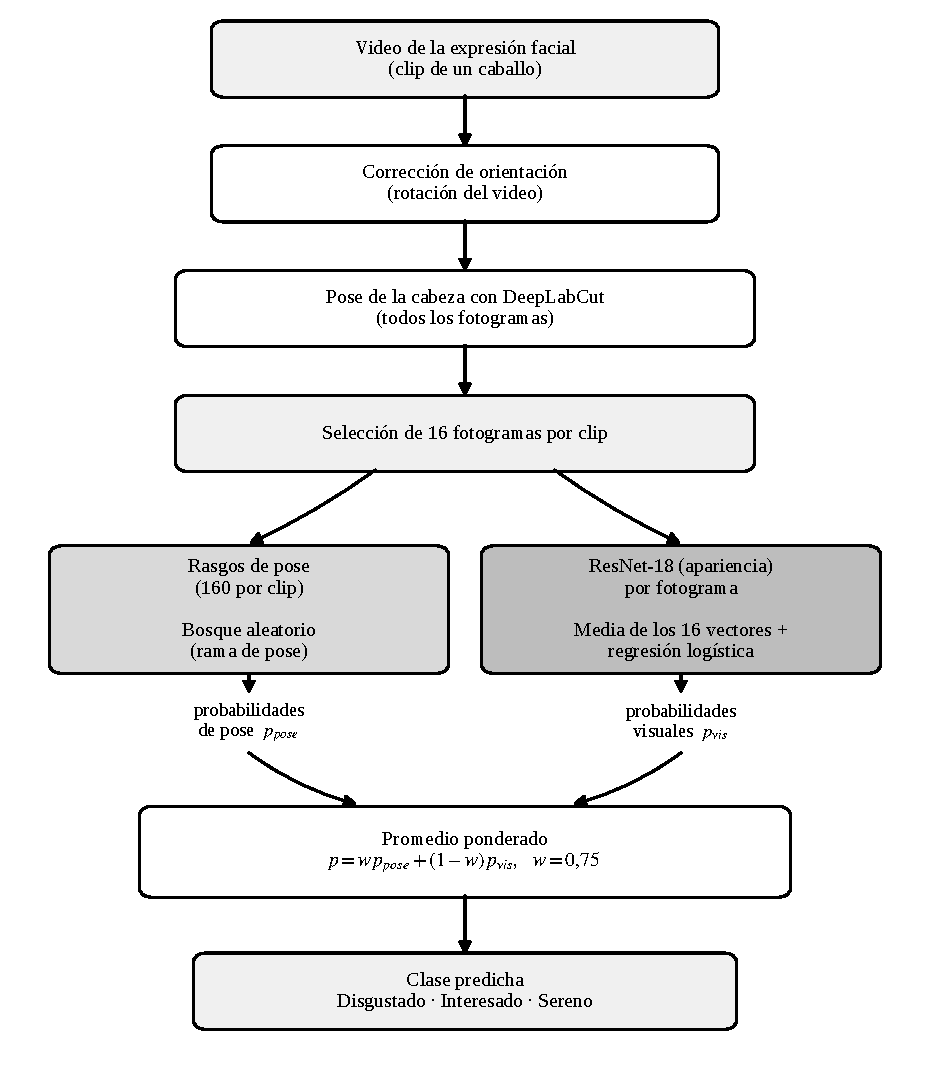
\includegraphics[width=\textwidth]{figuras/pipeline.pdf}
\notatabla{Los \PoseRasgos{} rasgos de pose se calculan con las coordenadas de DeepLabCut; la rama visual usa ResNet-18 sobre \Fotogramas{} fotogramas por clip. El peso de la pose, $w$ = \PesoPose{}, se elige por validación interna (\PesoPose{} en \PesoFoldsA{} de \PesoFoldsTotal{} pliegues).}
\end{figure}

\subsection{Orientación del Video}
Muchos teléfonos guardan el video sin rotar y registran la orientación como metadato. De los \VideosTotal{} videos, 69 tienen una rotación de 90 grados. Si el decodificador la ignora, el detector recibe la cara acostada y falla; en una medición temprana, los videos rotados perdían más de la mitad de sus fotogramas medidos. Se resolvió activando la corrección automática de OpenCV (\texttt{CAP\_PROP\_ORIENTATION\_AUTO}) en todas las lecturas, tanto en el entrenamiento como en la aplicación.

\subsection{Estimación de Pose sobre Todos los Fotogramas}
DeepLabCut se ejecutó con el modelo SuperAnimal-Quadruped sin ajuste, sobre todos los fotogramas de los 393 clips candidatos (alrededor de 73\,000). Una versión temprana ubicaba la cabeza con un detector de objetos YOLO \parencite{redmon2016,jocher2024}; en la versión vigente el encuadre se calcula con el ojo y el hocico estimados por la pose y el detector no participa. No se usó el subconjunto específico para caballos (Horse-30) ni se midió la calidad de los puntos frente a una anotación humana del conjunto; ambas son limitaciones declaradas. Es la etapa más costosa, pero se ejecuta una sola vez y su resultado se almacena, lo que permite cambiar el criterio de selección de fotogramas sin repetir el cálculo.

\subsection{Selección de los 16 Fotogramas}
Una primera versión fijaba 16 posiciones equiespaciadas antes de saber qué fotogramas tenían mediciones válidas; un fotograma fallido se recuperaba por interpolación o anotación manual, y con ese enfoque sólo 153 de los 393 clips resultaban utilizables. La versión vigente invierte el orden: primero mide y después elige. El algoritmo (a) busca la ventana temporal más larga, de hasta 7~s, que contenga al menos \Fotogramas{} fotogramas válidos y ningún hueco sin medición mayor a 0,5~s; (b) distribuye \Fotogramas{} posiciones equiespaciadas en esa ventana, y (c) ancla cada posición al fotograma válido de mayor confianza dentro de una tolerancia de 0,10~s. No se interpolan puntos ni se anotan fotogramas a mano: si un clip no ofrece una ventana suficiente, se descarta. Este cambio elevó los clips utilizables de 153 a \ClipsTotal{} sin filmar videos nuevos. Un fotograma es válido cuando la confianza de ojo y hocico es de al menos 0,50, el mismo umbral que se usa para construir las máscaras de validez de los puntos faciales (un punto con confianza menor se considera ausente).

\subsection{Representación Visual}
Cada fotograma seleccionado se alinea a partir de la posición del ojo y del hocico, se recorta con un encuadre de $224 \times 343$ píxeles que incluye las orejas, se guarda en JPEG con calidad 95 y se procesa con una ResNet-18 \parencite{he2016} preentrenada en ImageNet \parencite{deng2009} y congelada, que produce 512 características por fotograma. Cada clip queda representado por una matriz de \Fotogramas{}$\times$512. La aplicación de inferencia reproduce exactamente este recorrido, incluida la compresión, para que el modelo reciba en producción la misma distribución de imágenes que en el entrenamiento. Se probó entrenar parcialmente la ResNet-18 y no se obtuvo mejora distinguible (Anexo~C), por lo que el extractor permanece congelado.

\subsection{Representación de Pose}
La rama de pose parte de las coordenadas de ojos, hocico, orejas, mandíbula y comisuras de los mismos \Fotogramas{} fotogramas y produce dos representaciones.

\textbf{Rasgos tipo SimBA (\PoseRasgos{} por clip).} Siguiendo el estilo de rasgos que calcula SimBA \parencite{goodwin2024} a partir de una tabla de puntos ---distancias, ángulos, razones, velocidades y aceleraciones, con estadísticos agregados---, se programaron rasgos propios, porque los extractores de SimBA no son aplicables a este esquema de puntos; por eso el informe los llama «rasgos tipo SimBA» y no SimBA. Se agrupan en 130 rasgos estáticos (26 series por fotograma resumidas con media, desvío, mínimo, máximo y rango), 21 dinámicos (7 series de velocidad y aceleración resumidas con media, desvío y máximo) y 9 de disponibilidad (qué fracción de los fotogramas tiene medido cada punto). Todas las longitudes se dividen por la escala del clip, definida como la mediana de la distancia ojo--hocico entre sus fotogramas válidos; así no hay estadística global y no se filtra información entre pliegues. Un punto con confianza menor de 0,50 se trata como ausente: alrededor del 14~\% de los valores falta y se imputa con la mediana del entrenamiento dentro de cada pliegue.

\textbf{Geometría v2 (17 columnas por fotograma).} Es la descripción que usa el MIL. Todo se expresa en el marco de la cabeza (eje $x$ del ojo al hocico, escala igual a esa distancia en el fotograma): largo y ángulo de cada oreja (4 columnas), vector hocico--mandíbula (2), ancho de boca (1), distancia interocular (1), escorzo (1), seno y coseno de la inclinación de la cabeza (2) y seis máscaras de validez con umbral de confianza de 0,50. La versión anterior (v1, 9 columnas) llevaba esencialmente un solo grado de libertad ---la inclinación de la cabeza--- y máscaras que valían 1 en todos los fotogramas por usar un umbral de confianza nulo; la v2 corrige ambas cosas. Es una descripción 2D de una cámara, por lo que depende del punto de vista, y no fue validada con un especialista.

\section{Los Cuatro Candidatos}
Se compararon cuatro modelos de complejidad creciente, todos con la misma entrada de datos, las mismas particiones y el mismo evaluador. La Tabla~\ref{tab:c4-candidatos} los resume, con su orden de simplicidad (1 = más simple), que es el que utiliza la regla de desempate del criterio de elección. Los hiperparámetros se fijaron antes de medir y no se ajustaron con ningún conjunto de prueba; los que se eligen dentro de un candidato se eligen con una validación interna.

\begin{table}[H]
\caption{Candidatos de la comparación}\label{tab:c4-candidatos}
{\singlespacing\small
\begin{tabularx}{\textwidth}{@{}clXlc@{}}
\toprule
N.º & Candidato & Descripción & Entrada & Simplicidad \\
\midrule
1 & Línea de base & Regresión logística sobre la media de los \Fotogramas{} vectores visuales & Visual & 1 \\
2 & Bosque aleatorio de pose & Bosque aleatorio (\textit{random forest}) sobre los \PoseRasgos{} rasgos tipo SimBA & Pose & 2 \\
3 & Fusión pose + visual & Promedio ponderado de las probabilidades de los dos anteriores & Pose y visual & 3 \\
4 & MIL multimodal corregido & Red con atención sobre los \Fotogramas{} fotogramas & Visual y pose & 4 \\
\bottomrule
\end{tabularx}}
\notatabla{La simplicidad es una escala ordinal fijada en el protocolo antes de comparar: cuenta qué tan simple es el modelo en cantidad de componentes y de parámetros y en la facilidad de explicar su salida.}
\end{table}

\subsection{Candidato 1. Línea de Base sobre la Media Visual}
Se promedian los \Fotogramas{} vectores de 512 características de cada clip, se estandarizan (media y desvío calculados sólo con el entrenamiento del pliegue) y se ajusta una regresión logística multinomial con regularización $C = 0{,}1$, pesos de clase balanceados y hasta 5\,000 iteraciones. Es el modelo más simple y ignora tanto el orden como la pose; sirve de referencia para saber qué aporta cada componente adicional.

\subsection{Candidato 2. Bosque Aleatorio de Pose}
Sobre los \PoseRasgos{} rasgos tipo SimBA se ajusta un bosque aleatorio \parencite{breiman2001} de 500 árboles, con \texttt{max\_features} igual a la raíz del número de rasgos, hojas de al menos 2 muestras (\texttt{min\_samples\_leaf} = 2), pesos de clase balanceados y semilla 0, precedido de una imputación por la mediana del entrenamiento. Estos hiperparámetros se habían fijado en la auditoría, antes de la comparación, y no se eligieron mirando datos de prueba.

\subsection{Candidato 3. Fusión Tardía de Pose y Apariencia}
La fusión combina las probabilidades de los dos modelos anteriores \parencite[fusión de clasificadores;][]{kittler1998}, según la ecuación~(\ref{eq:c3-fusion}) del Capítulo~3, con la notación siguiente:
\[
p = w\,p_{\mathrm{pose}} + (1-w)\,p_{\mathrm{visual}},
\]
donde $p_{\mathrm{pose}}$ es la salida del bosque aleatorio y $p_{\mathrm{visual}}$ la de la regresión logística. El peso $w$ pertenece al conjunto $\{0;\,0{,}25;\,0{,}5;\,0{,}75;\,1\}$ y se elige dentro de cada ajuste con una validación interna por caballo de 4 pliegues (\texttt{StratifiedGroupKFold}, semilla 0) sobre el entrenamiento, maximizando la \fmacro{} de las probabilidades fuera de muestra; si hay empate se prefiere el peso más cercano a 0,5. Una vez elegido $w$, ambos modelos se reentrenan con todo el entrenamiento. La variante tardía se fijó antes de mirar resultados de prueba y la variante temprana (concatenar rasgos) no se evaluó. En las 20 evaluaciones del desarrollo el peso elegido fue \PesoPose{} en \PesoFoldsA{} de \PesoFoldsTotal{} pliegues y \PesoPoseUno{} en el restante: la fusión está dominada por la pose.

\subsection{Candidato 4. MIL Multimodal Corregido}
Es el modelo con que se trabajó hasta el 07/10, con tres correcciones que surgieron de la auditoría: geometría v2 en lugar de v1, máscaras de validez con umbral 0,50 y validación interna estratificada por caballo y por clase. En el aprendizaje con múltiples instancias \parencite{ilse2018} cada clip es una «bolsa» de \Fotogramas{} fotogramas y el modelo aprende cuánto pesa cada uno. La arquitectura es la siguiente: por cada fotograma, el vector geométrico de 17 columnas pasa por un perceptrón multicapa $17 \rightarrow 64 \rightarrow 128$ con activaciones ReLU y se concatena con las 512 características visuales (640 dimensiones); una red de atención ($640 \rightarrow 128 \rightarrow 1$, con tangente hiperbólica) asigna un puntaje a cada fotograma, que una softmax con máscara convierte en pesos; la suma ponderada forma la representación del clip, que un clasificador $640 \rightarrow 64 \rightarrow 3$ convierte en puntajes por clase. Tiene 132\,867 parámetros entrenables, sin contar la ResNet-18. Como la atención es una suma ponderada, el modelo es invariante al orden de los fotogramas: se verificó numéricamente que barajar o invertir los \Fotogramas{} fotogramas no cambia ninguna de las \ClipsTotal{} predicciones, de modo que agrega información de varias imágenes pero no modela la evolución temporal.

La Tabla~\ref{tab:c4-hiper} reúne los hiperparámetros de entrenamiento.

\begin{table}[H]
\caption{Hiperparámetros del MIL multimodal corregido}\label{tab:c4-hiper}
{\singlespacing
\begin{tabular}{@{}ll@{}}
\toprule
Parámetro & Valor \\
\midrule
Optimizador & Adam, tasa de aprendizaje $10^{-3}$, decaimiento de pesos $10^{-4}$ \\
Tamaño del lote & 32 \\
Pérdida & Entropía cruzada con pesos de clase inversos a la frecuencia \\
\textit{Dropout} & 0,0 \\
Épocas máximas / paciencia & 100 / 10 \\
Criterio de parada & \fmacro{} en la validación interna \\
Validación interna & 25~\% del entrenamiento, por caballo, estratificada por clase \\
Punto de control conservado & El de mayor \fmacro{} en validación \\
Semilla & 42 \\
Geometría y máscaras & v2 (17 columnas), umbral de confianza 0,50 \\
\bottomrule
\end{tabular}}
\notatabla{Los pesos de clase se calculan sobre el entrenamiento interno. La parada temprana \parencite{prechelt2012} se decide con la validación interna; el conjunto de prueba del pliegue no interviene.}
\end{table}

\section{Protocolo de Evaluación}
El protocolo se escribió y se versionó antes de medir ningún candidato (\texttt{comparacion/PROTOCOLO.md}). Toda modificación posterior a la visión de resultados debía registrarse como enmienda con fecha. La pregunta que responde es cuál de los candidatos clasifica mejor la expresión en caballos nunca vistos, sin que la ventaja pueda explicarse por rasgos de filmación. Se agrupó por caballo porque un mismo animal aparece en varios clips, y repartirlos entre entrenamiento y prueba permitiría al modelo reconocer al individuo en lugar de la expresión \parencite{kapoor2023,varoquaux2018}.

\subsection{Reserva}
Antes de cualquier comparación se apartó una reserva del 15~\% de los caballos: \CaballosReserva{} caballos con \ClipsReserva{} clips, sorteados con semilla fija (20261007) y estratificados por la clase dominante de cada caballo (la de más clips; en caso de empate, la más rara). Los \CaballosDesarrollo{} caballos restantes (\ClipsDesarrollo{} clips) forman el \textit{desarrollo}. La reserva no se usa para elegir hiperparámetros, umbrales, épocas ni arquitectura, ni para mirar curvas. El único acceso es una función que exige una autorización explícita y un motivo, registra cada uso en un archivo de bitácora y se niega a un segundo uso: el cerrojo es mecánico y no una promesa. La reserva se usó una sola vez, con el ganador, después de registrar por escrito la decisión. Con \CaballosReserva{} caballos el intervalo resultante es ancho, y el número no se emplea para comparar candidatos.

\subsection{Particiones y Validación Interna}
En el desarrollo se usan 5 repeticiones $\times$ 4 pliegues (5$\times$4) por caballo con \texttt{StratifiedGroupKFold}, con barajado y semillas 1101 a 1105, persistidas en un archivo versionado. Son \Evaluaciones{} evaluaciones por candidato y todos usan exactamente las mismas. Aserciones del código verifican que ningún caballo cruza entrenamiento y prueba, que la reserva no aparece y que cada pliegue de prueba contiene las tres clases. Todo ajuste propio de un candidato ---hiperparámetros elegidos, época, peso $w$--- se hace dentro del entrenamiento de cada evaluación, con una validación interna por caballo; está prohibido elegir con el pliegue de prueba \parencite{cawley2010}.

\subsection{Métricas e Incertidumbre}
La métrica principal es la \fmacro{} \parencite{sokolova2009}, que da el mismo peso a las tres clases; se informa la media y el desvío de las \Evaluaciones{} evaluaciones y, por repetición, el \fmacro{} agrupado de las predicciones fuera de muestra. Además se calculan la exactitud, la precisión, la sensibilidad (\textit{recall}) y el \textit{F}\textsubscript{1} por clase, las matrices de confusión, la \fmacro{} en el subconjunto limpio (por repetición) y la brecha entre la \fmacro{} de entrenamiento y la de prueba, como indicador de sobreajuste. Las repeticiones remuestrean la partición pero no los datos, así que su desvío no es un error estándar. Para la incertidumbre de una diferencia entre candidatos se usa un bootstrap \parencite{efron1993} pareado por caballo: se remuestrean con reposición los caballos del desarrollo, arrastrando todos sus clips, y en cada una de las \ReplicasBootstrap{} réplicas (semilla \SemillaBootstrap{}) se calcula la diferencia de \fmacro{} entre ambos candidatos; se informa el intervalo del 95~\%. Lo mismo se hace sobre el subconjunto limpio.

\subsection{Criterio de Elección}
El criterio de elección, fijado antes de comparar, tiene tres reglas que se aplican en orden:

\begin{enumerate}
  \item \textbf{Ordenamiento.} Es líder el candidato con mayor \fmacro{} media sobre las \Evaluaciones{} evaluaciones del desarrollo.
  \item \textbf{No inferioridad en el subconjunto limpio.} El candidato elegido no puede ser inferior a ningún otro en el subconjunto limpio, entendiendo por inferior que el límite superior del intervalo de la diferencia (candidato menos otro) sea menor que cero. Si el líder la incumple, pasa a evaluarse el siguiente del ranking.
  \item \textbf{Empate.} Se considera empatado con el líder a todo candidato cuyo intervalo de la diferencia en desarrollo contra el líder incluye el cero. Entre los empatados gana el más simple (Tabla~\ref{tab:c4-candidatos}).
\end{enumerate}

El resultado completo se registra aunque haya un ganador claro y no se descarta a ningún candidato por razones distintas de estas.

\subsection{Enmienda: Validación Dejando Afuera una Sesión}
Los límites declarados en el protocolo incluían que el agrupamiento por caballo no impide que caballos de una misma sesión queden de lados distintos, de modo que condiciones de filmación compartidas podrían favorecer la evaluación. El 08/10/2026, antes de correr el análisis, se declaró una enmienda con un análisis complementario de validación dejando afuera una sesión de filmación: sobre los \ClipsDesarrollo{} clips del desarrollo, para cada una de las \SesionesEvaluadas{} sesiones con clips de desarrollo, el conjunto de prueba son los clips de esa sesión y el de entrenamiento son los clips de las demás sesiones, \textit{excluyendo} los de cualquier caballo presente en la sesión de prueba (así no hay fuga ni por sesión ni por caballo). Esa exclusión quitó \ClipsTrainPerdidos{} clips de entrenamiento en total (\ClipsTrainPerdidosMedia{} por sesión en promedio); el entrenamiento de cada sesión quedó entre \ClipsTrainSesionMin{} y \ClipsTrainSesionMax{} clips. Los cuatro candidatos se evalúan con la misma partición y los mismos hiperparámetros ya fijados, con un candidato nuevo por sesión. Como muchas sesiones tienen pocos clips o una sola clase, la métrica es la \fmacro{} agrupada sobre todas las predicciones fuera de muestra, con el intervalo bootstrap por caballo. El análisis no cambia la elección del ganador, que ya estaba fijada, ni toca la reserva; si contradijera la elección, se registraría como limitación. El resumen fiel del protocolo y de su enmienda está en el Anexo~B.

\section{Evolución del Desarrollo}
El trabajo no siguió el orden en que se lo presenta aquí. La Tabla~\ref{tab:c4-hitos} resume los hitos y la presente sección explica por qué el eje del informe cambió de un modelo a una comparación.

\begin{table}[H]
\caption{Hitos principales del desarrollo}\label{tab:c4-hitos}
{\singlespacing\small
\begin{tabularx}{\textwidth}{@{}p{2.6cm}X@{}}
\toprule
Fecha (2026) & Hito \\
\midrule
Mayo & Plan de trabajo, objetivos e hipótesis general. \\
13--21/08 & Primer \textit{pipeline} (preparación del conjunto, detección y pose con DeepLabCut); diagnóstico de cobertura, orientación y encuadre. \\
28/08--05/09 & Primeras evaluaciones sobre 141 y 153 clips; modelo de promedio con \fmacro{} 0,704. \\
15/09 & Modelo MIL multimodal. \\
17--23/09 & Auditoría del \textit{pipeline}; selección por ventana temporal (\ClipsTotal{} clips), validación interna y parada temprana; ablaciones. \\
25/09 & Líneas de base del conjunto vigente, control del confusor de filmación y registro del sobreajuste. \\
28/09--07/10 & Protocolo de etiquetado; equivalencia entre entrenamiento e inferencia; auditoría v2 y experimento con rasgos tipo SimBA. \\
07/10 & Protocolo de comparación declarado antes de medir; apartado de la reserva. \\
08/10 & Los cuatro candidatos, decisión del ganador, único uso de la reserva, validación por sesión y verificación de la identidad 123/169. \\
\bottomrule
\end{tabularx}}
\end{table}

\textbf{Del MIL a la comparación.} El desarrollo comenzó con un modelo de promedio de fotogramas y evolucionó hacia el MIL multimodal con atención, con la hipótesis de que el orden y el aporte de cada fotograma capturaban la dinámica de la expresión. En el protocolo de entonces, con 4 pliegues por caballo y sin repeticiones, el MIL alcanzó una \fmacro{} de 0,740 ± 0,052. Entre el 17/09 y el 07/10 se lo sometió a una auditoría del \textit{pipeline} y del protocolo, que reveló cuatro cosas: (a) el orden temporal no aportaba, pues el modelo es invariante a él; (b) una línea de base estática, el promedio de fotogramas con regresión logística, igualaba su rendimiento (0,741); (c) existían confusores de filmación ---la duración y el formato del clip predecían la clase---; y (d) el criterio de aceptación (0,691) se había definido sobre otro conjunto y otra línea de base. Un experimento sugerido por el docente, la clasificación con rasgos tipo SimBA, mostró que un bosque aleatorio sobre la pose superaba al MIL en el mismo protocolo (0,841), con la alerta de que esos rasgos también predicen la duración del clip.

\textbf{Devolución del docente.} El profesor Juan Toloza anotó el informe de cumplimiento de condiciones con dieciséis observaciones, que se agruparon en comentarios escritos, una nota sobre SimBA, una nota de diagnóstico con cinco indicaciones y pasajes resaltados sin comentario. Algunas se resolvieron con una medición (la invariancia al orden, la línea de base estática, el sobreajuste), otras con un cambio de método (el criterio declarado de antemano, el subconjunto limpio, la validación por sesión), y otras sólo se pudieron atender en parte o quedó abierta. La tabla completa, con la acción y el resultado de cada una, está en el Anexo~D. La consecuencia principal fue declarar la hipótesis temporal como no sostenida y reorientar el trabajo desde «mejorar el MIL» hacia «elegir el mejor clasificador con un protocolo común y honesto», que es el protocolo descrito arriba.

\textbf{Caminos explorados.} Antes y durante este proceso se probaron 47 caminos ---variantes de datos, de representación, de modelo, de validación, de entorno y de aplicación---, adoptados, reemplazados o descartados, cada uno con su motivo. Se resumen en el Anexo~C; ninguno de los descartados fue ocultado y varios (como la geometría v2 o los rasgos tipo SimBA) pasaron a ser componentes de los candidatos finales.

\section{Aplicación de Inferencia}
Se implementó una aplicación web con Streamlit (\texttt{app\_inferencia.py}) que sólo se ocupa de la presentación: la lógica vive en el módulo \texttt{equinos/inferencia.py}, que reutiliza el código de selección de fotogramas, alineación y extracción del entrenamiento. Una prueba automatizada verifica sobre clips reales que ambas ramas eligen los mismos fotogramas y producen recortes idénticos píxel a píxel; esa prueba detectó durante el desarrollo un cambio de umbral que había desalineado la aplicación respecto del modelo entrenado.

El modelo que sirve por omisión es la fusión tardía de pose y apariencia, ganadora de la comparación. Se entrenó una vez con los \ClipsTotal{} clips (desarrollo y reserva), con el peso $w$ = \PesoPose{}, sin calcular ninguna métrica sobre los clips con que se lo entrena: la confiabilidad que se muestra es la medida fuera de muestra (desarrollo y reserva). El modelo anterior (MIL) queda disponible como opción explícita. Se guarda un paquete con los dos modelos, el peso, las clases y los metadatos (versión de scikit-learn, huella del conjunto, fecha y lista de clips).

La aplicación procesa un video nuevo en tres etapas (ubicación de la cara y los puntos clave en cada fotograma, selección de los \Fotogramas{} fotogramas y clasificación) y presenta:
\begin{itemize}
  \item un aviso inicial, visible sin buscarlo, de que no es un instrumento de diagnóstico veterinario, con el nivel de acierto en la reserva y sus limitaciones;
  \item la clase estimada, la confianza del modelo en este video y, en lenguaje llano, cuánto se puede confiar en esa respuesta, a partir de la precisión medida por clase (un rango cuando el desarrollo y la reserva no coinciden);
  \item las probabilidades por clase y la explicación de cómo se llegó a la respuesta: qué opinó cada una de las dos lecturas (postura de la cara y aspecto de la imagen) y si coinciden o no;
  \item el \textit{tramo analizado}: segundo de inicio y de fin de la ventana de a lo sumo 7~s sobre la que se clasificó y duración total del video; si éste es más largo, recomienda subir una toma recortada al momento de interés.
\end{itemize}

La negativa es una respuesta de primera clase. El modelo consume clips íntegros de \Fotogramas{} fotogramas alineados, y sobre el conjunto propio sólo el 91,3~\% de los clips candidatos los ofrece; para un video cualquiera, no responder es un resultado esperable. Cuando el ojo y el hocico no pueden medirse durante un tramo continuo, o el video supera la duración máxima admitida (15~s), la aplicación se niega a clasificar y explica el motivo, en lugar de dar una etiqueta cuya confiabilidad nadie midió. Los textos se redactaron para una persona que no leyó el informe y se revisaron con una persona ajena al proyecto (n = 1); no se realizó ninguna validación con veterinarios ni un test externo, por lo que la utilidad para el público objetivo no está medida. Las pantallas y los textos se describen en el Anexo~F.

% ============================================================
% CAPÍTULO 5
% ============================================================
\capitulo{Resultados y Discusión}

\section{Rendimiento del Modelo}
Sobre 359 clips de 133 caballos, el modelo MIL multimodal obtuvo un \fmacro{} de 0,740 ($DE = 0{,}052$ entre particiones; IC 95~\% por \textit{bootstrap} de caballos [0,677; 0,797]) y una exactitud de 0,744. Supera el criterio de aceptación fijado antes de entrenar (0,691). La Tabla~\ref{tab:porclase} detalla las métricas por clase y la Tabla~\ref{tab:confusion}, la matriz de confusión.

\begin{table}[H]
\caption{Métricas por clase del modelo MIL multimodal}\label{tab:porclase}
{\singlespacing
\begin{tabular}{@{}lrrrr@{}}
\toprule
Clase & Precisión & Sensibilidad & \textit{F}\textsubscript{1} & \textit{n} \\
\midrule
\clase{Disgustado} & 0,740 & 0,689 & 0,714 & 103 \\
\clase{Interesado} & 0,764 & 0,797 & 0,780 & 118 \\
\clase{Sereno} & 0,729 & 0,739 & 0,734 & 138 \\
\bottomrule
\end{tabular}}
\notatabla{Predicciones fuera de muestra de las cuatro particiones agrupadas por caballo.}
\end{table}

\begin{table}[H]
\caption{Matriz de confusión del modelo MIL multimodal}\label{tab:confusion}
{\singlespacing
\begin{tabular}{@{}lrrr@{}}
\toprule
& \multicolumn{3}{c}{Clase predicha} \\
\cmidrule(l){2-4}
Clase real & \clase{Disgustado} & \clase{Interesado} & \clase{Sereno} \\
\midrule
\clase{Disgustado} & 71 & 13 & 19 \\
\clase{Interesado} & 5 & 94 & 19 \\
\clase{Sereno} & 20 & 16 & 102 \\
\bottomrule
\end{tabular}}
\end{table}

El error dominante es la confusión entre \clase{Sereno} y \clase{Disgustado} (20 y 19 clips), más frecuente que la que parecería semánticamente más cercana. Algunos caballos son clasificados mal en todos sus clips; un error sistemático sobre un mismo animal es más compatible con una etiqueta discutible o con una apariencia atípica que con ruido del modelo, pero sin una segunda opinión sobre las etiquetas no es posible distinguir entre ambas causas.

\section{Variabilidad entre Particiones}
El \fmacro{} de prueba fue de 0,718, 0,769, 0,677 y 0,795 en las cuatro particiones. La dispersión indica que el rendimiento depende de qué caballos quedan en prueba, lo esperable cuando el tamaño efectivo de la muestra son 133 animales y no 359 clips independientes.

\section{Líneas de Base}
La Tabla~\ref{tab:lineas} compara el modelo con las líneas de base evaluadas sobre las mismas particiones.

\begin{table}[H]
\caption{Comparación con líneas de base}\label{tab:lineas}
{\singlespacing
\begin{threeparttable}
\begin{tabular}{@{}lrr@{}}
\toprule
Modelo & \fmacro{} (\textit{DE}) & Exactitud \\
\midrule
Clase mayoritaria & 0,183 (0,033) & 0,384 \\
Azar estratificado\tnote{a} & 0,325 (0,025) & --- \\
Duración del clip & 0,544 (0,035) & 0,532 \\
Geometría sola (media y desvío) & 0,607 (0,033) & 0,618 \\
Metadatos de filmación & 0,618 (0,034) & 0,635 \\
Visual, un fotograma central & 0,679 (0,024) & 0,688 \\
Visual, promedio de 16 fotogramas & 0,741 (0,020) & 0,749 \\
MIL multimodal (modelo final) & 0,740 (0,052) & 0,744 \\
\bottomrule
\end{tabular}
\begin{tablenotes}[flushleft]\footnotesize
\item[a] Esperanza del \fmacro{} de predicciones aleatorias con las proporciones de clase; percentil 95: 0,367.
\end{tablenotes}
\end{threeparttable}}
\notatabla{Todas las líneas de base son regresiones logísticas evaluadas con las mismas cuatro particiones por caballo que el modelo final. \textit{DE} = desvío estándar entre particiones.}
\end{table}

Tres resultados se desprenden de la comparación. Primero, el modelo supera con amplitud al azar y a la clase mayoritaria. Segundo, los metadatos de filmación por sí solos alcanzan 0,618: la forma en que se filmó cada clase contiene señal. El modelo los supera por 0,121 (IC 95~\% [0,031; 0,211]), de modo que su rendimiento no se reduce a esos metadatos. Tercero, y más importante, un clasificador lineal sobre el \textit{promedio} de las características visuales de los 16 fotogramas obtiene 0,741, prácticamente lo mismo que el modelo final: la diferencia es de $-0{,}005$ con IC 95~\% [$-0{,}068$; 0,058], que incluye el cero. Usar 16 fotogramas sí aporta respecto de uno solo (diferencia de 0,059, IC 95~\% [0,001; 0,116]), pero no se demuestra que la atención, la geometría ni el orden agreguen algo sobre un resumen estático de esos fotogramas.

\section{Control del Contexto de Filmación}
Para estimar cuánto del rendimiento depende de rasgos de la filmación, se restringió la evaluación a los clips que comparten resolución ($1080 \times 1920$) y tienen al menos 5~s de duración, sin reentrenar. Sobre esos 236 clips el modelo conserva un \fmacro{} de 0,705 y una exactitud de 0,746. El subconjunto contiene sólo 28 clips de \clase{Disgustado}, por lo que el resultado es indicativo; aun así, la caída es moderada y sugiere que el modelo no depende principalmente de la duración ni de la resolución.

Este control no alcanza al contexto que la etiquetadora describe (box de hipódromo para \clase{Interesado}, interacción en manada para \clase{Disgustado}). Que la clase se asocie al entorno es inherente al fenómeno, pero el modelo puede aprovecharlo como pista: los videos con varios animales en cuadro pertenecen casi siempre a \clase{Disgustado} y el modelo los clasifica mejor que al resto de esa clase.

\section{Sobreajuste}
El registro por época del entrenamiento interno muestra un sobreajuste marcado: el \fmacro{} medio fue de 0,979 en entrenamiento, 0,712 en validación y 0,740 en prueba (Anexo~C). La parada temprana contiene el problema: el rendimiento de prueba se mantiene en línea con el de validación. Con 132\,355 parámetros y unos 200 clips de entrenamiento por partición, la memorización del conjunto de entrenamiento es esperable.

\section{Evaluación de la Hipótesis Temporal}
La hipótesis temporal no queda respaldada. La GRU y la atención con codificación posicional, sensibles al orden, no superaron de manera consistente a las variantes invariantes. En el modelo de promedio, permutar los fotogramas no cambia el resultado por construcción, y el modelo final, cuya atención no usa la posición, es igualmente invariante al orden. La comparación con el promedio estático refuerza la conclusión: un resumen sin orden ni atención alcanza el mismo rendimiento.

La conclusión es acotada. No implica que la dinámica sea irrelevante en la expresión equina ---en dolor equino se reportó lo contrario \parencite{broome2019}---, sino que \textit{con este conjunto, esta ventana de hasta 7~s y estas representaciones, no se encontró evidencia de que el orden de los 16 fotogramas mejore la clasificación}.

\section{Variantes No Adoptadas}
El ajuste fino parcial de la ResNet18 (última etapa convolucional) obtuvo 0,747 ($DE = 0{,}057$), una diferencia pequeña frente a la variabilidad entre particiones que no justificaba el costo ni el riesgo adicional de sobreajuste. Tampoco mejoraron el modelo un canal geométrico con más puntos anatómicos, puntos de boca y ollares, la validación cruzada anidada para elegir la época, el enmascarado de clips incompletos ni una representación del movimiento de la cabeza. La geometría resultó útil sólo como complemento: el MIL visual sin geometría obtuvo 0,686.

\section{Limitaciones}
\begin{enumerate}
  \item \textbf{Un único observador.} El acuerdo se midió en un piloto sobre imágenes, no sobre este conjunto. Se desconoce el techo de rendimiento que impone la ambigüedad de las etiquetas.
  \item \textbf{El criterio de etiquetado no es sólo facial.} Incluye ambiente, comportamiento y postura, información a la que el modelo, que ve un recorte de la cara, no accede por completo.
  \item \textbf{Asociación entre clase y contexto.} La clase se relaciona parcialmente con el establecimiento, la situación y la duración de la toma.
  \item \textbf{Tamaño efectivo.} Los 133 caballos limitan la precisión de las estimaciones, como muestra la variabilidad entre particiones.
  \item \textbf{Sin validación externa.} No se evaluó el modelo con videos de otras fuentes, cámaras o regiones.
  \item \textbf{Validación interna pequeña.} La elección de la época se apoya en pocos caballos por partición.
  \item \textbf{Pose sin adaptación.} DeepLabCut se usa sin entrenamiento adicional sobre este conjunto.
  \item \textbf{Costo de inferencia.} Procesar un video nuevo demora de uno a tres minutos con GPU.
\end{enumerate}

\section{Discusión General}
Los resultados muestran que la cara del caballo, tal como la captura un video corto de celular, contiene señal suficiente para discriminar las tres clases definidas en el conjunto, y que esa señal se generaliza a animales no vistos durante el entrenamiento. El rendimiento es comparable entre clases y supera claramente a las líneas de base que no miran la cara.

Al mismo tiempo, el trabajo muestra que la complejidad del modelo no fue lo que determinó el resultado. Los avances más grandes provinieron de decisiones metodológicas: eliminar la fuga por identidad, corregir la orientación de los videos, ampliar el encuadre para incluir las orejas, rediseñar la selección de fotogramas y unificar entrenamiento e inferencia. Un clasificador lineal sobre un resumen estático de varios fotogramas iguala a la arquitectura final. Con un conjunto de este tamaño, la calidad de los datos y el control de sesgos pesan más que la arquitectura.

% ============================================================
% CAPÍTULO 6
% ============================================================
\capitulo{Conclusiones}

\section{Cumplimiento de los Objetivos}
\subsection{Conjunto de Datos}
Se conformó un conjunto propio de 274 videos y 393 clips de equinos, de los cuales el sistema utiliza 359, correspondientes a 133 caballos, con un criterio de etiquetado documentado y referido a EquiFACS.

\subsection{Preprocesamiento}
Se implementó un \textit{pipeline} reproducible que estima la pose, elige una ventana temporal medida, selecciona 16 fotogramas, alinea la cara y genera representaciones visuales y geométricas, con un aprovechamiento del 91,3~\% de los clips.

\subsection{Clasificación}
El modelo MIL multimodal alcanza un \fmacro{} de 0,740 y una exactitud de 0,744 con evaluación agrupada por caballo, por encima del criterio de aceptación fijado de antemano.

\subsection{Aplicación}
Se implementó una aplicación de inferencia que usa el mismo código que el entrenamiento, verificado por pruebas automatizadas, y que se niega a clasificar cuando el video no permite una medición suficiente.

\section{Conclusión sobre la Hipótesis General}
La hipótesis general se considera respaldada dentro de los límites del conjunto: es factible clasificar automáticamente las tres expresiones definidas a partir de videos cortos, con generalización a caballos no observados y un rendimiento por encima del criterio establecido. La afirmación se refiere a las categorías y al criterio de una etiquetadora; no constituye una validación clínica ni etológica externa.

\section{Conclusión sobre la Hipótesis Temporal}
La hipótesis temporal no fue demostrada. Los modelos sensibles al orden no superaron a los invariantes, y un resumen estático de los 16 fotogramas alcanza el mismo rendimiento que el modelo final. Utilizar varios fotogramas sí resultó útil; ordenarlos o ponderarlos, no.

\section{Aportes}
\begin{itemize}
  \item Un conjunto de datos propio de expresiones faciales equinas con criterio de etiquetado documentado.
  \item La identificación y el control de la fuga de información por identidad.
  \item Un método de selección de fotogramas que mide antes de elegir y más que duplicó el aprovechamiento de los clips.
  \item Un sistema de líneas de base que permite atribuir el rendimiento a sus fuentes y detectar atajos.
  \item La equivalencia verificada entre el procesamiento de entrenamiento y el de inferencia.
  \item El registro de resultados negativos y de variantes descartadas.
\end{itemize}

\section{Trabajo Futuro}
\begin{enumerate}
  \item Medir el acuerdo entre observadores sobre una muestra del conjunto: que una segunda persona etiquete a ciegas unos 60 clips con el criterio documentado y se calcule el $\kappa$ de Cohen \parencite{cohen1960}.
  \item Incorporar más caballos, en particular de \clase{Disgustado} en contextos distintos de la manada.
  \item Validar el modelo con videos de otras fuentes y establecimientos.
  \item Equilibrar el contexto de filmación entre clases o controlarlo explícitamente.
  \item Estudiar representaciones temporales sólo si nuevos datos muestran señal temporal que el esquema actual no captura.
  \item Reducir el costo de la estimación de pose en inferencia.
\end{enumerate}

\section{Conclusión Final}
Un sistema de clasificación de expresiones faciales equinas puede construirse con un \textit{pipeline} reproducible y evaluarse con rigor evitando la fuga por identidad. El mejor resultado no provino de aumentar la complejidad del modelo sino de mejorar el aprovechamiento de los datos, la coherencia metodológica y el control de sesgos. La información de varios fotogramas resulta útil, pero con los datos y escalas estudiados no se encontró evidencia de que su orden sea determinante. El trabajo futuro debería orientarse a ampliar y diversificar el conjunto y a medir la confiabilidad de sus etiquetas antes que a arquitecturas temporales más complejas.

% ============================================================
% CAPÍTULO 7 — BIBLIOGRAFÍA
% ============================================================
\clearpage
\chapter*{Bibliografía}
\addcontentsline{toc}{chapter}{Capítulo 7. Bibliografía}
\begingroup
\setlength{\bibhang}{1.27cm}
\printbibliography[heading=none]
\endgroup

% ============================================================
% CAPÍTULO 8 — ANEXOS
% ============================================================
\clearpage
\chapter*{Anexos}
\addcontentsline{toc}{chapter}{Capítulo 8. Anexos}

\section{Anexo A. Parámetros del Sistema}
\begin{table}[H]
\caption{Parámetros principales}\label{tab:parametros}
{\singlespacing
\begin{tabularx}{\textwidth}{@{}lX@{}}
\toprule
Parámetro & Valor \\
\midrule
Fotogramas por clip & 16 \\
Ventana temporal máxima & 7,0~s \\
Hueco máximo entre mediciones & 0,5~s \\
Tolerancia de anclaje & 0,10~s \\
Confianza mínima de ojo y hocico & 0,50 \\
Tamaño del recorte & $224 \times 343$ píxeles \\
Extractor visual & ResNet18 preentrenada en ImageNet, congelada \\
Dimensión visual / geométrica & 512 / 9 \\
Proyección geométrica & $9 \rightarrow 64 \rightarrow 128$ \\
Particiones externas & 4, agrupadas por caballo \\
Épocas máximas / paciencia & 100 / 10 \\
Épocas del modelo de producción & 29 \\
Parámetros entrenables & 132\,355 \\
\bottomrule
\end{tabularx}}
\end{table}

\section{Anexo B. Componentes del Software}
\begin{itemize}
  \item \texttt{equinos/catalogo.py}: catálogo de videos por clase.
  \item \texttt{equinos/reproceso.py}: estimación de pose sobre todos los fotogramas.
  \item \texttt{equinos/secuencia.py}: selección temporal de fotogramas.
  \item \texttt{equinos/alineado.py}: alineación de la cara.
  \item \texttt{equinos/dataset.py}: construcción de los recortes.
  \item \texttt{equinos/caracteristicas.py}: extracción con ResNet18.
  \item \texttt{equinos/clasificacion.py}: modelo, entrenamiento y evaluación.
  \item \texttt{equinos/particion.py}: particiones por caballo.
  \item \texttt{equinos/inferencia.py} y \texttt{app\_inferencia.py}: aplicación de inferencia.
  \item \texttt{scripts/evaluar\_v2.py} y \texttt{scripts/evaluar\_lineas\_de\_base.py}: evaluación del modelo y de las líneas de base.
  \item \texttt{tests/}: pruebas automatizadas, entre ellas la de equivalencia entre entrenamiento e inferencia.
\end{itemize}

\section{Anexo C. Resultados por Partición}
\begin{table}[H]
\caption{Entrenamiento, validación y prueba por partición}\label{tab:folds}
{\singlespacing
\begin{tabular}{@{}rrrrr@{}}
\toprule
Partición & Mejor época & \textit{F}\textsubscript{1} entrenamiento & \textit{F}\textsubscript{1} validación & \textit{F}\textsubscript{1} prueba \\
\midrule
1 & 28 & 0,973 & 0,700 & 0,718 \\
2 & 26 & 0,994 & 0,766 & 0,769 \\
3 & 20 & 0,969 & 0,641 & 0,677 \\
4 & 40 & 0,981 & 0,742 & 0,795 \\
\midrule
Media & 28,5 & 0,979 & 0,712 & 0,740 \\
\bottomrule
\end{tabular}}
\notatabla{\textit{F}\textsubscript{1} macro. El entrenamiento se evalúa sin \textit{dropout} con los pesos de la mejor época.}
\end{table}

\section{Anexo D. Variantes Evaluadas}
\begingroup\singlespacing\small
\setlength{\LTleft}{0pt}
\begin{longtable}{@{}p{0.27\textwidth}p{0.42\textwidth}p{0.23\textwidth}@{}}
\caption{Modelos y variantes evaluados}\label{tab:modelos}\\
\toprule
Modelo & Descripción & Resultado \\
\midrule
\endfirsthead
\toprule
Modelo & Descripción & Resultado \\
\midrule
\endhead
Un fotograma y voto & Regresión logística por fotograma y voto entre 16 predicciones. & 0,660 sobre 153 clips. \\
Modelo de promedio & Proyección compartida y promedio de 16 fotogramas. & 0,704 sobre 153 clips. \\
GRU & Recurrente, sensible al orden. & No superó a los invariantes. \\
Atención con posición & Atención con codificación posicional. & Sin mejora consistente. \\
CNN--LSTM & ResNet18 seguida de LSTM. & No integrada. \\
MIL visual & MIL sólo con características visuales. & 0,686. \\
MIL multimodal & Visual, geometría y atención. & Modelo final: 0,740. \\
Ajuste fino parcial & Última etapa de la ResNet18 entrenable. & 0,747; no adoptado. \\
Canal geométrico ampliado & Más puntos anatómicos. & Peor o más inestable. \\
Puntos de boca y ollares & Puntos faciales adicionales. & Sin mejora. \\
\bottomrule
\end{longtable}
\endgroup

\end{document}
